% !TEX program = lualatex
\PassOptionsToPackage{table}{xcolor}
%\PassOptionsToPackage{draft}{graphicx}
\documentclass{matthijs}
\graphicspath{{../assets/}{./docs/assets/}{./docs/internship-report/}}

\begin{filecontents*}[overwrite]{\jobname.xmpdata}
	\Title{Internship Report}
	\Subject{Reflection on the project results}
	\Author{Matthijs Bakker}
	\Language{en-US}
	\Keywords{internship\sep final\sep written\sep report}
\end{filecontents*}

% BEGIN preamble.tex

% Style for first and last page
\usepackage{wallpaper}
\usepackage{color}
\definecolor{arobsblue}{HTML}{0e335c}

% Versioning plugin that retrieves data from the git repo dir
% Needs the "gitInfoHead" file to be generated, make sure
% that the shim script or the git hook is enabled
\usepackage[maxdepth=2]{gitinfo2}

% Use biblatex with biber backend for bibliography
\usepackage{csquotes}
\usepackage[style=ieee]{biblatex}
\renewcommand*{\mkbibacro}[1]{#1}
\setcounter{biburllcpenalty}{7000}
\setcounter{biburlucpenalty}{8000}

% This lets the text look really juicy
\usepackage{microtype}
\usepackage{extdash}

% A column for right-aligned autowrap text
\newcolumntype{R}{>{\arraybackslash}m{10cm}}

% PDF-A
\usepackage{colorprofiles}
\usepackage[a-3b]{pdfx}
\hypersetup{
	bookmarks=true,
	unicode=false,
	pdftoolbar=true,
	pdfmenubar=true,
	colorlinks=true,
	linkcolor=black,
	citecolor=black,
	filecolor=black,
	urlcolor=black
}
%\hypersetup{
%	colorlinks=true,
%	linkcolor=gray,
%	urlcolor=gray,
%	citecolor=gray
%}

% END preamble.tex


\usepackage{titlepage}
\usepackage{ragged2e}

\addbibresource{ir.bib}

% Typography
\babelfont{tt}{Inter-Regular}
\babelfont{rm}{Merriweather-LightItalic}
\usepackage{lettrine}

\definecolor{arobs blue}{HTML}{0e2642}
\definecolor{arobs comp}{HTML}{422a0e}
\definecolor{invisible}{rgb}{1,1,1}

% Page numbering
\usepackage{titlesec}
\usepackage{titletoc}
\usepackage{fancyhdr}
\usepackage{lastpage}
\pagestyle{fancy}
\fancyhf{}
\fancyhead{}
\renewcommand{\headrulewidth}{0pt}
\lfoot{\textcolor{invisible}{\gitAbbrevHash~\gitAuthorName~\gitAuthorIsoDate}}
\rfoot{\textbf{\thepage}\hspace{1ex}of\hspace{1ex}\pageref{LastPage}}

\usepackage{tikz}
\usepackage{tikzscale}
%\usepackage{tikz-uml}
\usetikzlibrary{positioning, arrows.meta, calc, decorations.text}

%\usepackage{tabularx}

\titleformat{\section}{\Large\bfseries\rmfamily\lsstyle\color{arobsblue}}{\thesection}{1.1em}{} [{\vspace{4pt}\titlerule[0.75pt]}]
\titleformat{\subsection}{\large\bfseries\rmfamily\lsstyle\color{arobsblue}}{\thesubsection}{1.1em}{} [{\vspace{4pt}\titlerule[0.75pt]}]
\titleformat{\subsubsection}{\normalsize\bfseries\ttfamily}{\thesubsubsection}{0.5em}{} [{\vspace{4pt}\titlerule[0.75pt]\vspace{-0.2em}}]

\usepackage{siunitx}
\sisetup{detect-all}
\sisetup{output-decimal-marker = {,}}

\renewcommand{\LettrineFontHook}{\rmfamily}

\begin{document}

	% Set language to English
	\taal{en}

	\maketitlepage{Internship Report}{1.0}
	\pagenumbering{arabic}
	\thispagestyle{empty}
	
	\lefthyphenmin=3
	\righthyphenmin=3
	\setcounter{tocdepth}{2}

	\begin{hoofdstuk*}{Summary}

		\setlength\parindent{1.5em}
		\setlength{\parskip}{0.5em plus 0.2em minus 0.1em}
		\linespread{1.2}
		
		\lettrine[findent=0.3em, nindent=0.0em, lraise=0.03]{R}{esearch} conducted in the US by the National Highway Traffic Safety Administration in 2016 found that 94 percent of all motorvehicle accidents that year could be attributed to human error \cite{nhtsa2017fatal}.
		Twenty-one percent of these accidents were so-called ``run-off-road crashes.''
		This type of accident involves a single vehicle veering off the road and colliding with a natural or artificial object \cite{liu2009factors}.
		The most common causes were driver intoxication and fatigue \cite{nhtsa2017fatal}.

		The automotive department of AROBS is on a mission to enable vehicles to be more autonomous.
		By requiring less human input, cars can drive in a more predictable and safer manner.
		AROBS has been developing an Advanced Driver-Assistance System (ADAS) that consists of numerous subsystems which warn the driver of danger on the road.
		One of these subsystems is called the Lane Departure Warning System (LDWS).
		It predicts when the vehicle is about to leave the road lane and propagates a warning to the ADAS so that precautionary measures can be taken to prevent incidents like run-off-road crashes.

		In order to detect the road lane that the vehicle is driving in, the LDWS analyzes video footage from a camera mounted on the dashboard.
		Resource demanding image processing techniques are run on a Graphical Processing Unit (GPU) integrated in the vehicle's onboard computer to scan for road lane markings and to predict the position of the car.
		The GPUs used for this purpose are expensive and power-inefficient, raising the total cost of the system.

		Due to a global chip shortage since the start of the COVID-19 pandemic, the prices of semiconductors have spiked \cite{ivanova2021chip}.
		In particular, the prices of GPUs have surged up to 150 percent of their list price \cite{cheng2021chip}.
		This has led chip consumers like AROBS to explore alternative technologies.
		A popular alternative that can empower high-bandwidth image processing technologies are Field Programmable Gate Arrays (FPGAs.)
		Whereas GPUs are multipurpose devices which can programmed for many different tasks, FPGAs have to be specifically designed to do one single task.
		The FPGA designer has fine-grained control over the layout of the FPGA, enabling the possibility to create devices that are tailored for a specific use case.
		An FPGA can be designed to do parallel tasks like video processing at a high bandwidth and low power draw, making is suitable for being integrated in embedded systems.

		The goal of my internship was to create a road lane marking detection system at a lower production cost and higher power efficiency than existing systems.
		I accomplished this goal by creating an FPGA-centered system that uses digital logic for its video processing task and a CPU for its decision making.
		The integration with other subsystems and devices is made possible through a UART interface.
		The device can process a video frame in 11.2 milliseconds and has an average power draw of 2.246 Watt.
		Compared to a popular GPU-oriented alternative, the Nvidia Jetson Nano, the system is four times more power efficient, 20 percent faster, and the production cost is seven times lower.
		A drawback of the system is that the lane marking detection does not work well under certain environmental conditions.
		The accuracy of detection depends on the quality of the road surface and lane markings, and the absence of roadside artifacts.
		The detection is too unreliable for a finalized product.

	\end{hoofdstuk*}

	\begin{inhoudspagina}

	\end{inhoudspagina}

	\pagenumbering{arabic}

	\begin{hoofdstuk*}{Preface}

		\setlength\parindent{1.5em}
		\setlength{\parskip}{0.5em plus 0.2em minus 0.1em}
		\linespread{1.2}

		This document aims to summarize all that I have worked on for the last eighteen weeks and to put it in an easy-to-read format.
		I will describe the different stages of the internship project, from conceptualization to realization.
		The first chapter is mainly about the internship organization, the stakeholders and the issue context.
		From this chapter, the reader will be able to grasp the intent of the project and how we expected to take this market opportunity.
		To contrast the expectations with reality, the next chapter entails the final product that I delivered.
		The purpose of each deliverable is explained and the way that they together form the system is illustrated.

		Chapters three to seven are dedicated to the professional activities.
		They show that the level at which the project was executed meets the level that is expected of me.
		The first activity, Management and Control, entails aspects related to the approach of the project, like the planning, the sequence, and the version management.
		Next comes the chapter Analyze, in which I will reflect back on my activities during the research phase of the project.
		This phase was important to the project because it shaped my knowledge on image processing and was of massive support when implementing the algorithms on my own.
		The Advise chapter explains how I arrived at the conclusions that I made in the advisory report, and gives a discussion on the results of the project.
		As per the planning, I spent seven weeks on the realization of the product.
		This stage of the project is discussed in the Design and Implementation chapters of this document.

		Last but not least, I will reflect back on my personal development during this project.
		At the beginning of the internship I set out personal goals that I wanted to work on.
		Reflecting back on these goals gives me new insights and helps me improve myself for future endeavors.
		My time in Romania has shown me a lot about who I am and what my qualities are within this field of study, and I would like to share my experience in this chapter.
		
		I would like to give a special thanks to Cătălin for helping me find a place to stay, Ionut for being awesome, Alexandra for helping me at the company, Mr. Jeong for mentoring me, and Călin for being by my side throughout the journey!

	\end{hoofdstuk*}
	
	\begin{hoofdstuk}{Project Definition}

		\setlength\parindent{1.5em}
		\setlength{\parskip}{0.5em plus 0.2em minus 0.1em}
		\linespread{1.2}
		\vspace{-2.5ex}
		\begin{paragraaf}{The Organization}

			AROBS Group is an global organization with branches in Europe and Asia.
			It is most well known for developing the TrackGPS fleet management software, which is the most used vehicle monitoring software in Romania.
			Additionally, it provides custom software services in areas such as Automotive, Cybersecurity, Life Sciences and HR management.
			The workforce entails over one thousand employees across nineteen offices.

			\vspace{0.3ex}
			\begin{figuur}{External view of the Cluj Business Center}

				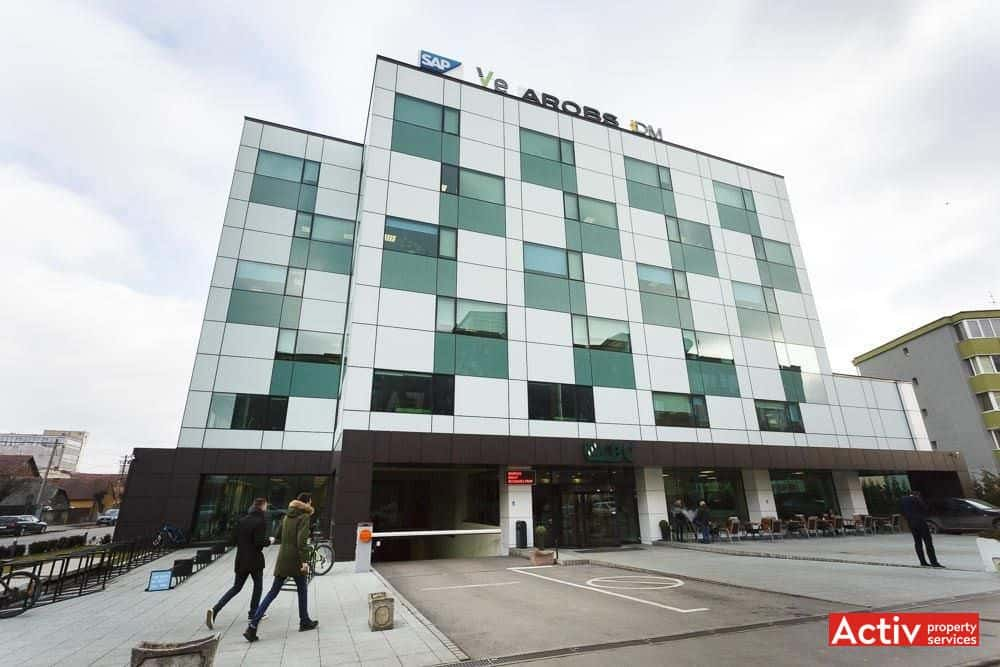
\includegraphics[width=0.75\textwidth, clip, trim=0cm 2cm 0cm 0cm]{cbc.jpg}

			\end{figuur}
			\vspace{-0.2ex}

			\noindent The primary office of AROBS is located in Cluj-Napoca, Romania. 
			It spans the second and third floor of the Cluj Business Center and houses a large part of the automotive department, consisting of over 400 employees.
			I spent most of my time working in the embedded department on the third floor of the building, where I was surrounded by friendly colleagues who were knowledgeable about anything from microcontrollers to FPGAs.
			
			Even though I was the only foreigner in the team, the atmosphere in the office was pleasant because I felt welcomed by my colleagues.
			They tried their best to speak English when I was around in order to include me in the conversation, which I really appreciated.
			My desk was next to a window with a beautiful view over the Baciu forest and its surrounding northern suburbs.
			A kitchen with the imperative coffee machine was just a small walk away from my desk.
			The business center also had facilities that I frequently made use of.
			Located on the first floor was a brunch restaurant from which a sweet smell emanated and filled the fitness center next to it.
			At the entrance was a coffee bar where I occasionally got my morning coffee.
			Once per month, a beer night was held to unite the department and encourage social activity among employees.
			I am left with the impression that AROBS is a modern company which invests in its employees by offering diverse activities.

			\noindent I was handed a laptop which I used for preparing documents and communicating with colleagues.
			Most internal communication at the company happened over Skype because it enabled inter-office messaging and helped to reach those who work at home.
			I was pleased with using Skype because I could instantly reach my company mentor and a few others who I was close with.
			It also allowed sending intermediate results during the development phase and getting feedback on them within a short timeframe.

			\vspace{1ex}
			\begin{figuur}{Organogram of AROBS Group}
				\centerline{
					\scalebox{0.9}{
				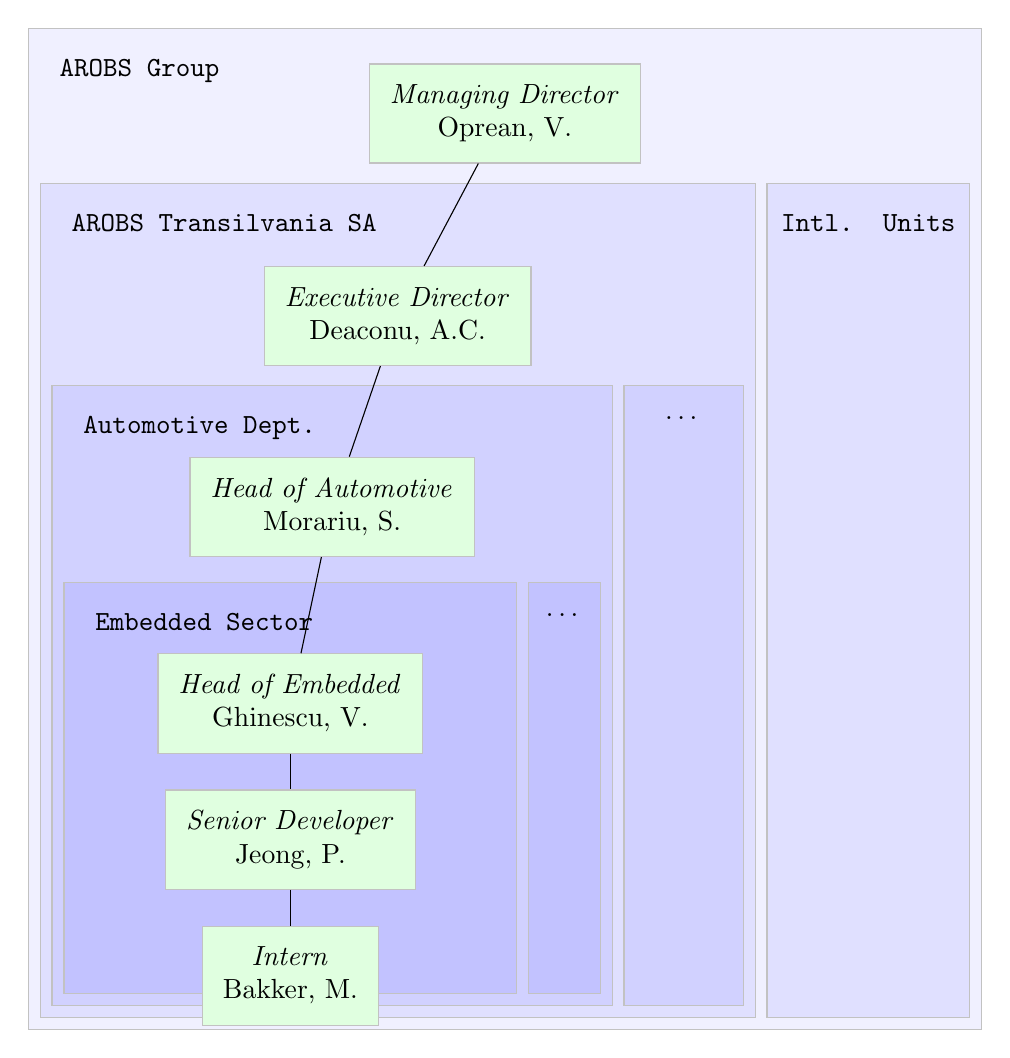
\begin{tikzpicture}
					
					\tikzstyle{grp}=[draw=black!24, align=right];
					\tikzstyle{man}=[draw=black!24, fill=green!12, align=center, inner sep=0.75em];

					\node (org) [grp, fill=blue!6, minimum width=80ex, minimum height=84ex, inner sep=0] {};
					\node (org label) [below right=0.8em and 0.8em of org.north west, align=left] {\ttfamily AROBS Group};
					\node (org man 1) [man, below=3ex of org.north] {\textit{Managing Director} \\ Oprean, V.};

					\node (rom) [grp, fill=blue!12, minimum width=60ex, minimum height=70ex, anchor=south west, above right=1ex and 1ex of org.south west, inner sep=0] {};
					\node (rom label) [below right=0.8em and 0.8em of rom.north west, align=left] {\ttfamily AROBS Transilvania SA};
					\node (rom man 1) [man, below=7ex of rom.north] {\textit{Executive Director} \\ Deaconu, A.C.};
					
					\node (oth) [grp, fill=blue!12, minimum width=17ex, minimum height=70ex, anchor=south east, above left=1ex and 1ex of org.south east, inner sep=0] {};
					\node (oth label) [below=0.8em of oth.north, align=center] {\ttfamily Intl. Units};

					\node (aum) [grp, fill=blue!18, minimum width=47ex, minimum height=52ex, anchor=south west, above right=1ex and 1ex of rom.south west, inner sep=0] {};
					\node (aum label) [below right=0.8em and 0.8em of aum.north west, align=left] {\ttfamily Automotive Dept.};
					\node (aum man 1) [man, below=6ex of aum.north] {\textit{Head of Automotive} \\ Morariu, S.};

					\node (otm) [grp, fill=blue!18, minimum width=10ex, minimum height=52ex, anchor=south east, above left=1ex and 1ex of rom.south east, inner sep=0] {};
					\node (otm label) [below=0.8em of otm.north, align=center] {\textellipsis};

					\node (emb) [grp, fill=blue!24, minimum width=38ex, minimum height=34.5ex, anchor=south west, above right=1ex and 1ex of aum.south west, inner sep=0] {};
					\node (emb label) [below right=0.8em and 0.8em of emb.north west, align=left] {\ttfamily Embedded Sector};
					\node (emb man 1) [man, below=6ex of emb.north] {\textit{Head of Embedded} \\ Ghinescu, V.};
					\node (emb man 2) [man, below=3ex of emb man 1.south] {\textit{Senior Developer} \\ Jeong, P.};
					\node (emb man 3) [man, below=3ex of emb man 2.south] {\textit{Intern} \\ Bakker, M.};
					
					\node (ots) [grp, fill=blue!24, minimum width=6ex, minimum height=34.5ex, anchor=south east, above left=1ex and 1ex of aum.south east, inner sep=0] {};
					\node (ots label) [below=0.8em of ots.north, align=center] {\textellipsis};

					\draw [-] (org man 1) -- (rom man 1);
					\draw [-] (rom man 1) -- (aum man 1);
					\draw [-] (aum man 1) -- (emb man 1);
					\draw [-] (emb man 1) -- (emb man 2);
					\draw [-] (emb man 2) -- (emb man 3);

				\end{tikzpicture}
					}
				}
			\end{figuur}
			\vspace{-0.2ex}

			\noindent I worked on the project alone, under the lead of my company mentor.
			We talked every Friday at 2 PM to discuss my progress and our expectations for next week.
			These meetings allowed me to give updates on the development progress and any roadblocks I was facing.
			Additionally, I reached out to my mentor over Skype when I had new results to show.
			For example, when I finally managed to get the detection working on the FPGA and I was ecstatic, I sent them the result video to share my excitement.

		\end{paragraaf}

		\begin{paragraaf}{The Project}

			One of AROBS' specialties is developing solutions for the automotive industry.
			Many of its clients have integrated the in-house developed Advanced Driver-Assistance System (ADAS) that aims to make cars more autonomous and relieve the driver of repetitive tasks.
			The value of automation in cars becomes clear when we view the statistics of road accidents: according to several studies \cite{nhtsa2017fatal} \cite{liu2009factors} \cite{dod2011run} conducted in the United States by the National Highway Traffic Safety Administration, \textit{human error} is the main factor in all fatal highway motorvehicle accidents.
			The study from 2016 shows that 94 percent of these were so-called "run-off-road crashes," which involved a single vehicle veering off the road and colliding with a natural or artificial object \cite{nhtsa2017fatal}.
			In these cases, the most common reason why the drivers lost control were intoxication and fatigue \cite{nhtsa2017fatal}.
			
			To take preventive measures against run-off-road crashes, the ADAS can be fitted with subsystems like a Lane Keeping System and a Lane Departure Warning System (LDWS).
			The latter is able to predict when a car is about to leave the lane and signal the ADAS of danger.
			Similarly to the stick shaker being activated in an aeroplane when it is about to stall, the car can notify the driver with a vibratory or auditory warning when it is unintentionally leaving the road lane.
			Other possible actions are automatically slowing down the car or correcting its course.

			In order to detect the position of the vehicle relative to the road lane, a video feed from the dashcam is processed by a computer vision algorithm.
			This algorithm is computationally expensive and requires to be run on an accelerated computing device like a Graphical Processing Unit (GPU.)
			Although lane detection systems using GPUs are widely used in prototypes and academic studies, they have failed to gain widespread adoption due to high production costs.
			Because GPUs are multipurpose devices that can be programmed to do many different tasks, they have been sought after by cryptocurrency miners, Machine Learning enthusiasts and big data hoarders, soaring the price up even higher.
			Since the start of the COVID-19 pandemic, the prices for GPUs have surged up to 150 percent of their list price due to factories not being able to produce them at full capacity \cite{cheng2021chip}.
			The increasing cost of these types of semiconductor devices has caused compaines like AROBS to consider replacing them with alternative hardware.
			
			Another device that can be programmed to process high amounts of data at once is a Field Programmable Gate Array.
			It is a chip that does not have a hardwired layout; it can be reconfigured to have different logic at any time.
			The chip is mass-produced in a "blank" state without any logic and the consumers can configure it to act like any digital logic circuit (as long as it fits on the chip's resources.)
			This means that an FPGA chip can be tailored to fit any use case.
			It also allows the FPGA designer fine-grained control over the chip's characteristics such as power draw and heat production.

			The core strength of an FPGA is parallel data processing.
			Digital logic circuits can be designed to have many signals that can work simultaneously, receiving the output of an operation on multiple data elements at the same time.
			In the field of image processing, this would mean that every pixel of an image could be processed simultaneously.
			A traditional processor would have to go over each pixel separately.

			I was assigned the task of creating an FPGA-based lane detection system that could outperform existing systems in terms of production cost per unit and power efficiency.
			With the market of hyper-autonomous cars being relatively new, this was a market opportunity that could have been seized.
			AROBS had previously built a GPU-based prototype system\,that was able detect road signs, objects and road lanes, which meant that there was a lot of knowledge in the company on the field of image processing.
			My mentor had worked on this prototype and was very knowledgeable on the subject of computer vision.
			With his help, it was my task to choose a sequence of algorithms that could be run on an FPGA and implement them in a proof-of-concept system.

			The initial situation was set out to be within the context of an existing vehicle.
			I assumed that systems for reading the dashcam footage and for propagating results to other ADAS subsystems for the car already existed.
			By placing them out of the scope of this project, I could focus my attention solely on developing the lane detector.

		\end{paragraaf}

		\begin{paragraaf}{Stakeholders}

			To make the project a success and meet the expectations of the parties who were involved with it, I had to make sure that each stakeholder's wishes would be satisfied.

			\vspace{2.5ex}
			\begin{figuur}{Stakeholder Analysis Matrix}
				\centerline{
				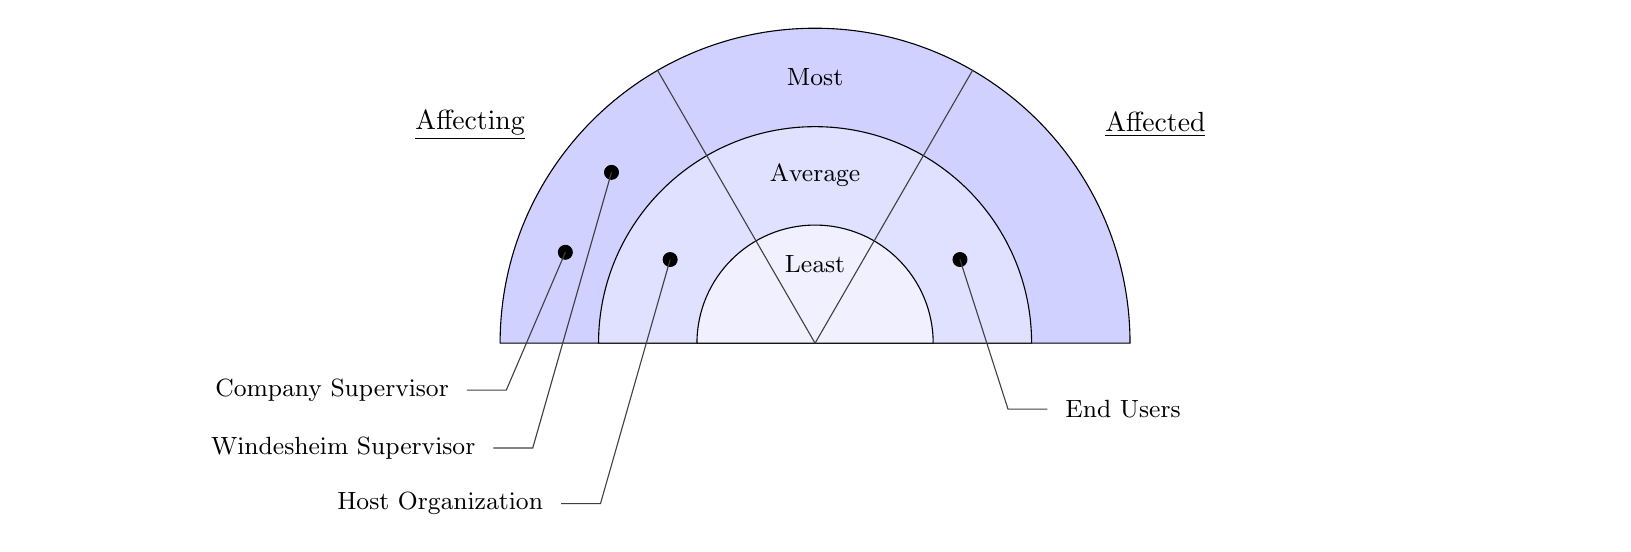
\begin{tikzpicture}[baseline=(current bounding box.north)]
					\path (-10, 0) -- (10, 0);
					\def\rad{4}
					\def\off{1.25}
					\def\offa{2.5}
					\draw [draw=black, fill=blue!18] (-\rad,0) -- (\rad,0) arc(0:180:\rad) --cycle;
					\draw [draw=black, fill=blue!12] (-\rad+\off,0) -- (\rad-\off,0) arc(0:180:\rad-\off) --cycle;
					\draw [draw=black, fill=blue!6] (-\rad+\offa,0) -- (\rad-\offa,0) arc(0:180:\rad-\offa) --cycle;
					%\draw [latex-latex] (-\rad, -0.5) -- (0, -0.5);
					\draw [color=darkgray] (0, 0) -- (60:\rad);
					\draw [color=darkgray] (0, 0) -- (120:\rad);

					\node[text centered] at (0, 1) {\small Least};
					\node[text centered] at (0, 2.125) {\small Average};
					\node[text centered] at (0, 3.375) {\small Most};
					\node[above right=2mm and 0.5cm of {(40:\rad)}, anchor=west] {\underline{Affected}};
					\node[above left=2mm and 0.5cm of {(140:\rad)}, anchor=east] {\underline{Affecting}};

					\coordinate (com sup p) at (160:\rad-\off/2);
					\coordinate (com sup s) at ($ (com sup p) + (-0.75, -1.75) $);
					\coordinate (com sup l) at ($ (com sup s) + (-0.5, 0) $);
					\filldraw (com sup p) circle (2.5pt);
					\draw [-, draw=darkgray] (com sup p)
						-- (com sup s)
						-- (com sup l);
					\node[left=0.7ex of com sup l, anchor=east] {\small Company Supervisor};

					\coordinate (win sup p) at (140:\rad-\off/2);
					\coordinate (win sup s) at ($ (win sup p) + (-1, -3.5) $);
					\coordinate (win sup l) at ($ (win sup s) + (-0.5, 0) $);
					\filldraw (win sup p) circle (2.5pt);
					\draw [-, draw=darkgray] (win sup p)
						-- (win sup s)
						-- (win sup l);
					\node[left=0.7ex of win sup l, anchor=east] {\small Windesheim Supervisor};

					\coordinate (host org p) at (150:\rad-\off-\off/2);
					\coordinate (host org s) at ($ (host org p) + (-0.885, -3.1) $);
					\coordinate (host org l) at ($ (host org s) + (-0.5, 0) $);
					\filldraw (host org p) circle (2.5pt);
					\draw [-, draw=darkgray] (host org p)
						-- (host org s)
						-- (host org l);
					\node[left=0.7ex of host org l, anchor=east] {\small Host Organization};
					
					\coordinate (end users p) at (30:\rad-\off-\off/2);
					\coordinate (end users s) at ($ (end users p) + (0.61, -1.9) $);
					\coordinate (end users l) at ($ (end users s) + (0.5, 0) $);
					\filldraw (end users p) circle (2.5pt);
					\draw [-, draw=darkgray] (end users p)
						-- (end users s)
						-- (end users l);
					\node[right=0.7ex of end users l, anchor=west] {\small End Users};

					%\draw [decorate, decoration={text along path, reverse path, raise=3ex, text={Affected}, text align={center}}] (\rad,0) arc(0:60:\rad);
					%\draw [decorate, decoration={text along path, raise=3ex, text={Affecting}, text align={center}}] (-\rad,0) arc(0:-60:-\rad);
				\end{tikzpicture}
				}
			\end{figuur}
			\vspace{-1ex}

			\noindent The above figure gives an overview of all stakeholders, along with their level of impact.
			It also shows whether a stakeholder has effect on the project or is affected by the outcome of the project.
			A brief description of each stakeholder and their interests is given in the following paragraphs.

			
			\begin{subparagraaf}{Host Organization}

				The organization instantiated this project and was the main driving force behind the resources of this project.
				It wanted to have evidence that FPGA-based technology could be used in this field by having a functional prototype.
				Although the organization was a secondary stakeholder, it could steer the project by giving the go/no go signal.
				It also purchased the hardware that I used to develop the system, which meant that it had financial resources invested and expected to see results from its investment.

			\end{subparagraaf}

			\begin{subparagraaf}{Company Supervisor}

				It was in the best interest of the company supervisor that I would deliver a working proof-of-concept system.
				Since the supervisor was my main point of contact within the company, I would be working with them closely, making them a high priority stakeholder.


			\end{subparagraaf}

			\begin{subparagraaf}{Windesheim Supervisor}

				This stakeholder was involved with giving approval of several deliverables, including the Plan of Action and the midterm presentation.
				The main requirement set by this stakeholder was that the project was complex enough to be on par with level two of the HBO-ICT competences.
				I planned to comply with this by realizing complex products, such as implementing the image processing techniques and continuously testing the deliverables.
				They expected me to send a progress report at the end of every week for keeping watch on the status of my project.

			\end{subparagraaf}

			\begin{subparagraaf}{End Users}

				The system is abstracted away in the car, making it not directly accessible by the consumers.
				However, they will be relying on the system to give accurate results in order to guarantee their safety.
				Therefore, this stakeholder desires the system to be able to detect danger in real-time with low latency and high precision.

			\end{subparagraaf}

		\end{paragraaf}

	\end{hoofdstuk}
	
	\begin{hoofdstuk}{The Product}

		\setlength\parindent{1.5em}
		\setlength{\parskip}{0.5em plus 0.2em minus 0.1em}
		\linespread{1.2}
		\vspace{-2.5ex}
		
		During the internship I created a prototype lane detector alongside tools that can interact with it.
		The lane detector itself is fully implemented on the TUL Z2 board.
		The tools are run on a personal computer or laptop that can be interfaced with it through a serial port.
		An example setup of the lane detector being interfaced with the Remote Control tool running on a mechanic's laptop can be seen in \verwijzingb{figuur}{Prototype Setup}.

		\begin{figuur}{Prototype Setup}
			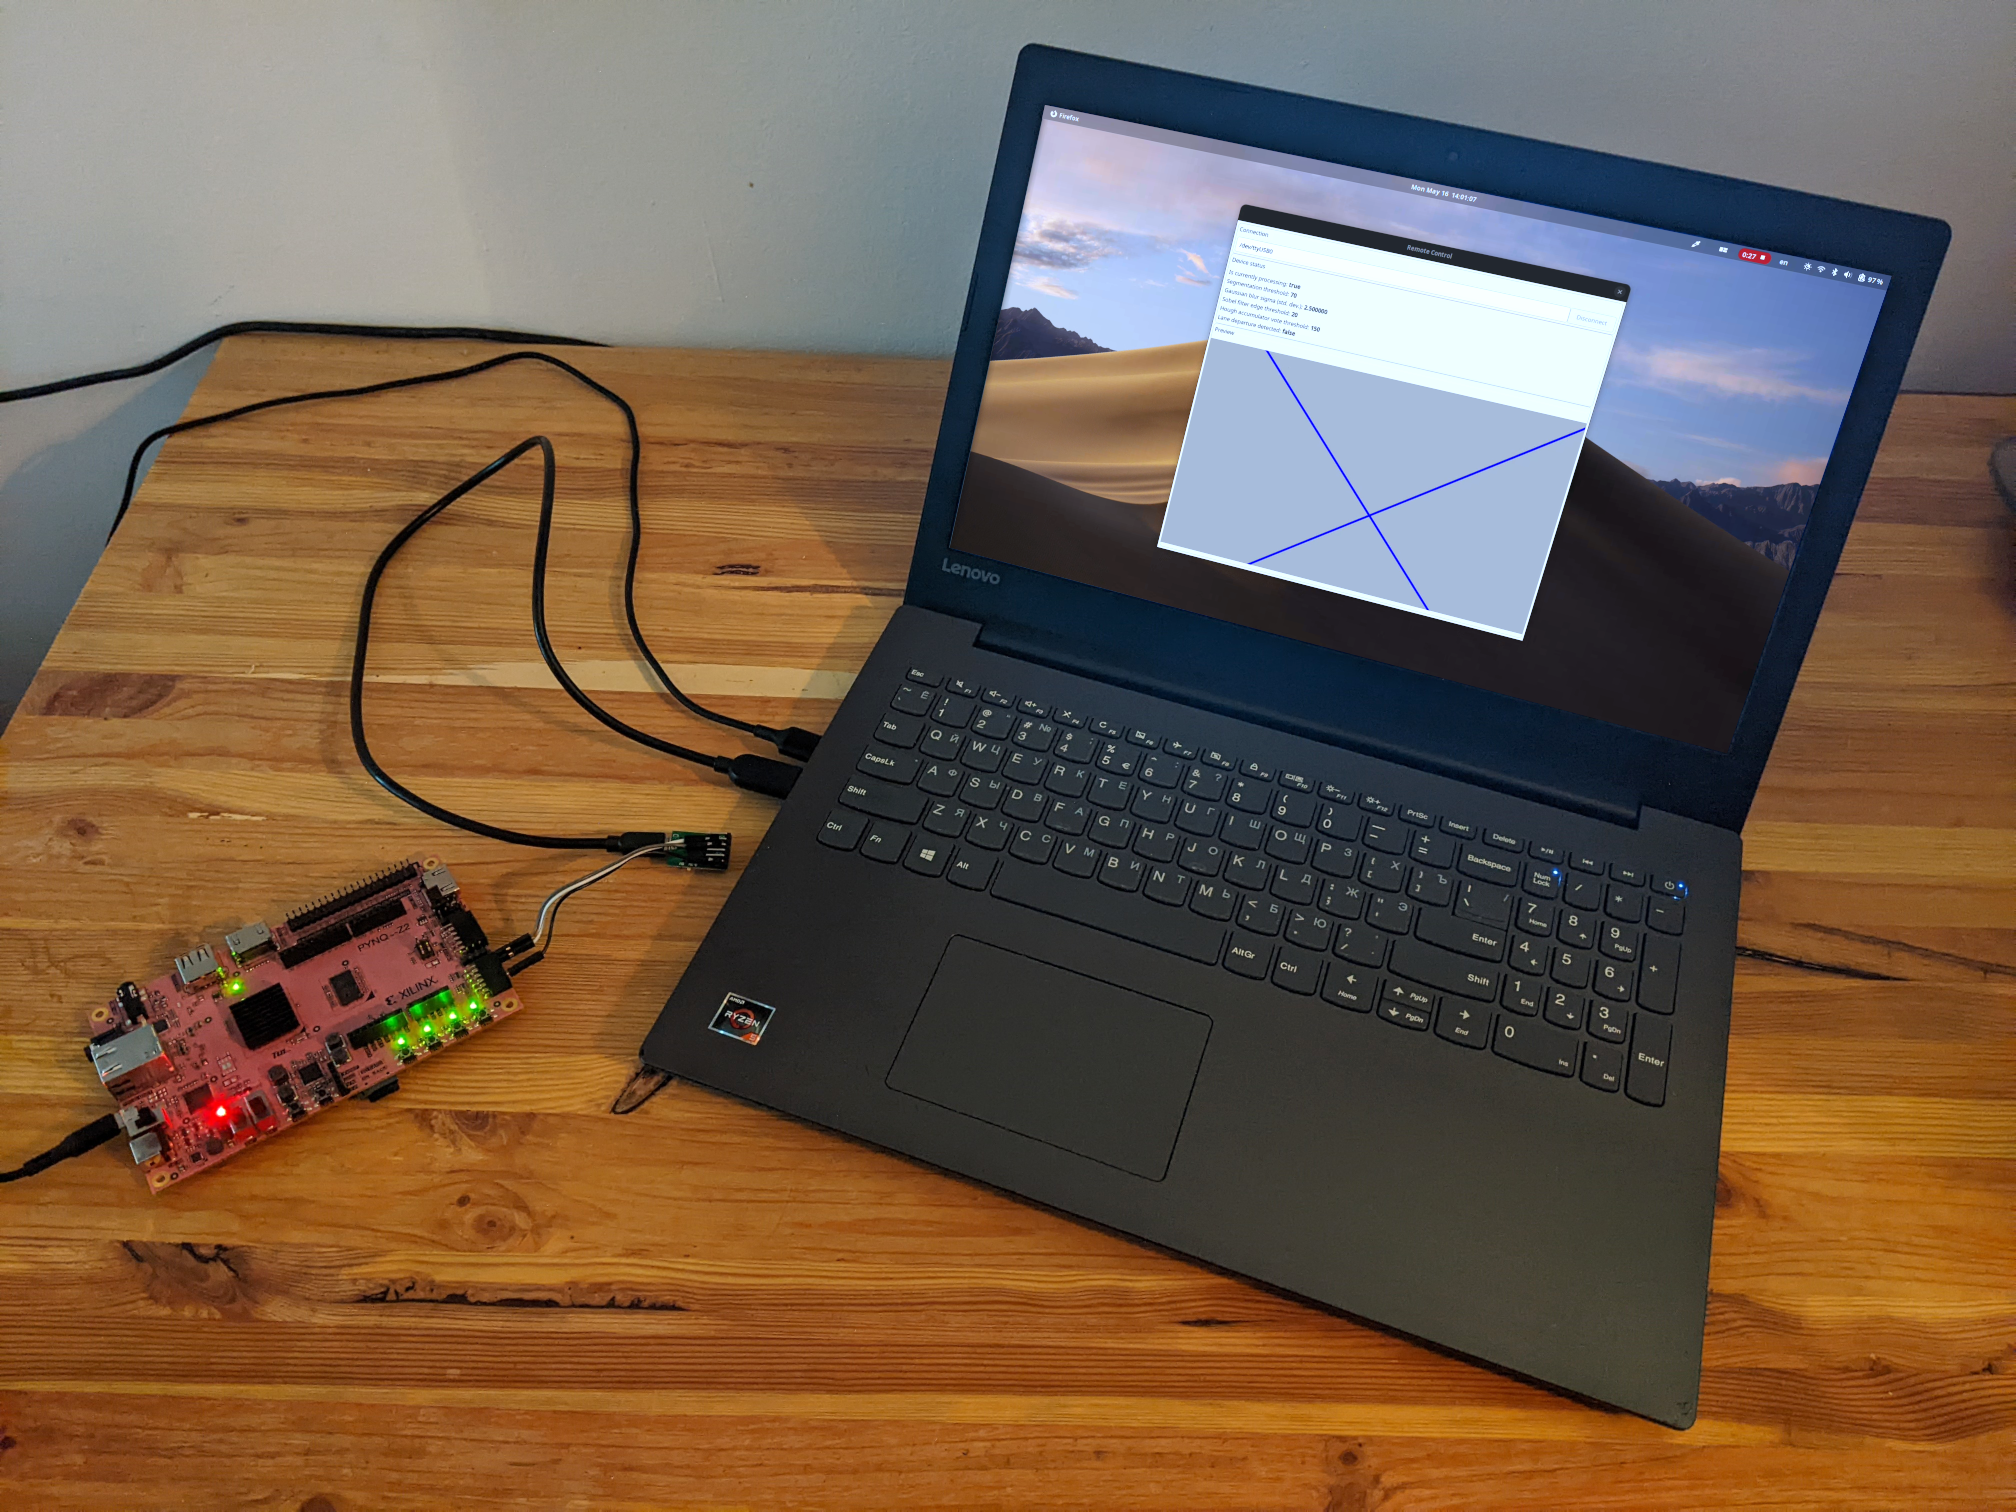
\includegraphics[width=0.8\textwidth]{product-5.png};
		\end{figuur}

		\noindent The total product can be distinguished into multiple deliverables that are able to be used together to form one functional system.
		An overview of this system is given in \verwijzingb{figuur}{Product Deliverables}.

		\begin{figuur}{Product Deliverables}
			\vspace{2ex}
			\centerline{
				\includegraphics{deliverables}
			}
		\end{figuur}

		\begin{paragraaf}{Lane Detector}

			The detector is a combined hardware/software solution that is implemented on the TUL Z2 development board.
			It takes a video feed from an external input source and processes it in real time, predicting whether the vehicle is about to depart the road lane.
			When the vehicle is predicted to leave the lane, the tri-color leds are toggled to shine red and a warning is given over an external interface.
			This makes the device easily integrateable with other car components.

			\begin{figuur}{TUL Z2 Development Board}
				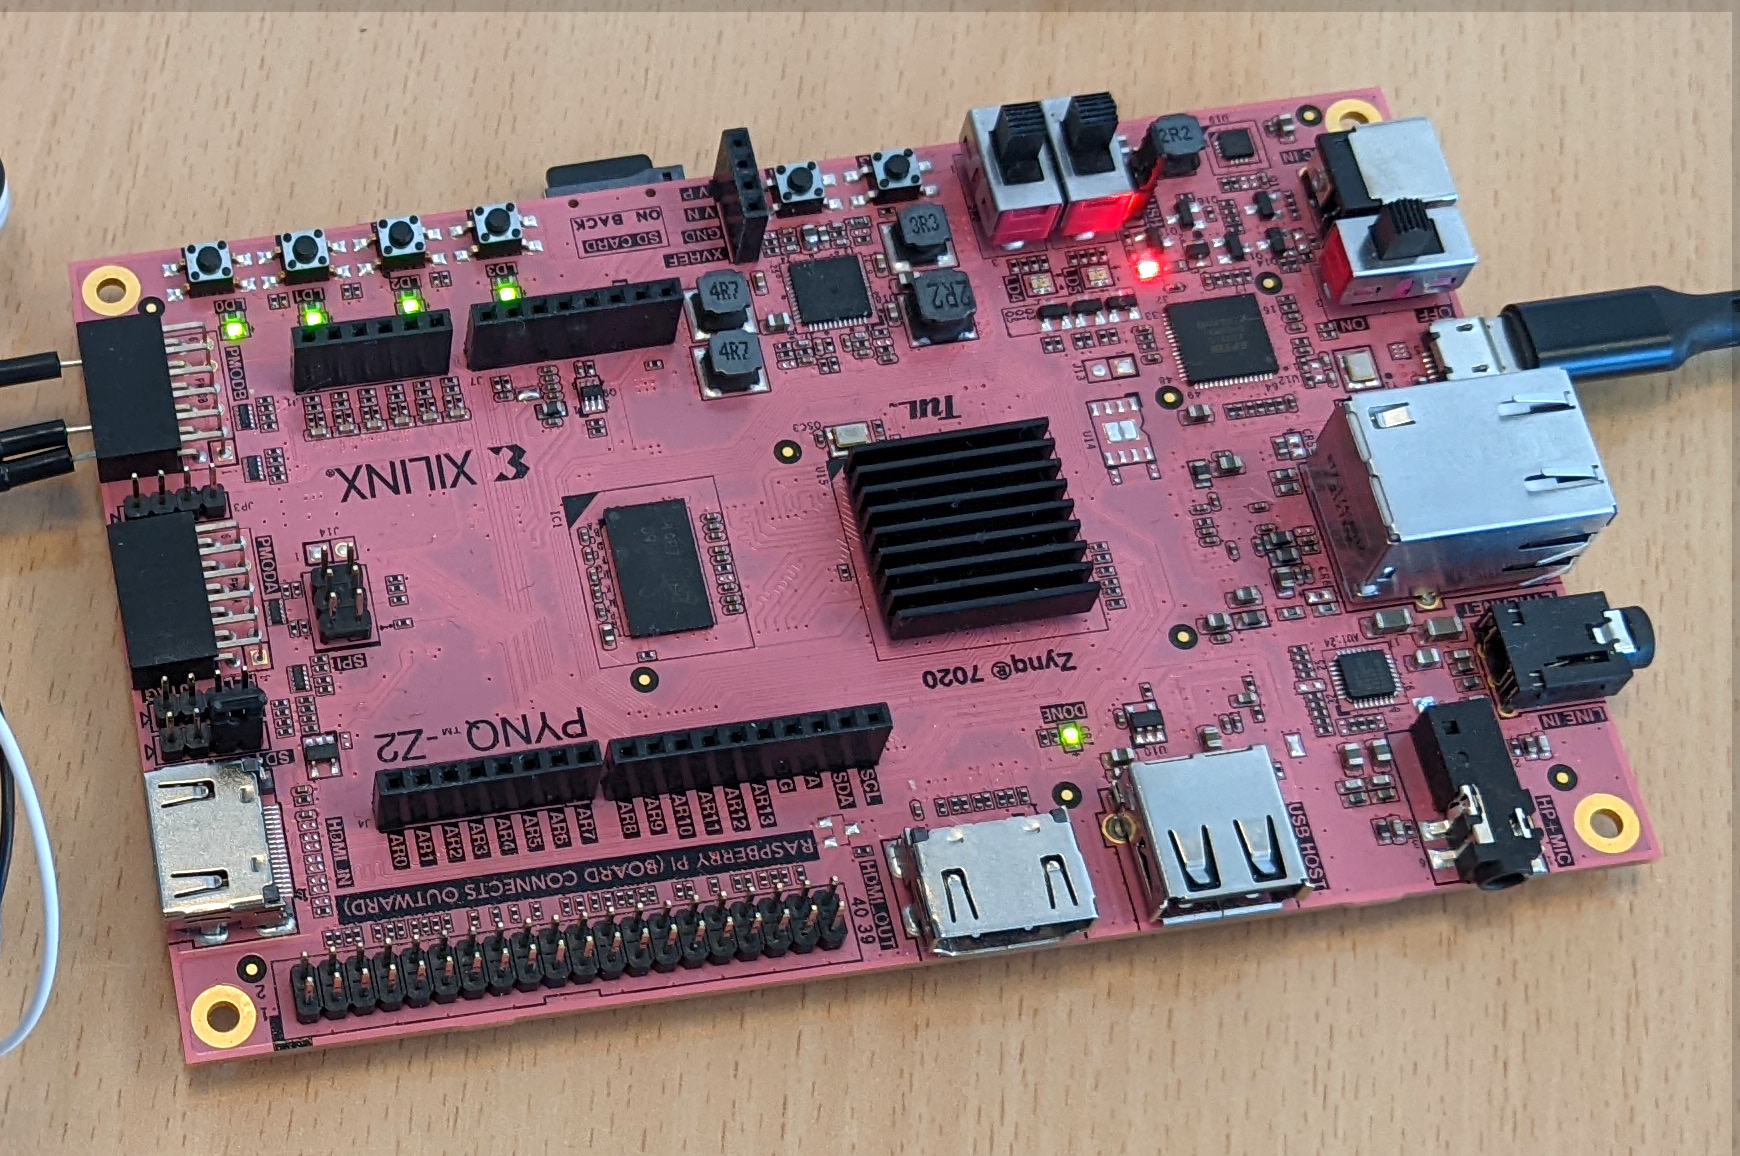
\includegraphics[width=0.8\textwidth]{product-6.png};
			\end{figuur}

			\noindent It takes 11.2 milliseconds for a video frame to be processed.
			The total latency between a video frame being received from the camera and the output of a lane departure warning is 26.6 milliseconds.
			This is fast enough to comply with the safety regulations and requirements as I set out in the functional design.
			The average power draw is 2.3 Watt, making it viable to implement in a battery powered vehicle.

		\end{paragraaf}

		\begin{paragraaf}{Remote Control Application}

			This application can be used on a mechanic's laptop to troubleshoot the lane detector.
			Algorithm settings and detection results that are broadcast over the external interface of the lane detector are received over the serial connection of the laptop and are read by the application.
			A graphical user interface (GUI) is shown to the mechanic which displays the settings and results of the lane detector.
			I developed this application to show that the results are correctly being sent over the lane detector's external serial interface and that other devices can reliably interface with it.
			It was also a good opportunity for me to debug the internals of the lane detector without connecting to it via the board's development framework.
			The application shows results in near real-time because of a fast serial data transfer rate, making it great for troubleshooting the device.
			As can be seen in \verwijzingb{figuur}{Remote Control User Interface}, the user interface shows all vital information about the lane detector to the mechanic.

			\vspace{1.5ex}
			\begin{figuur}{Remote Control User Interface}
				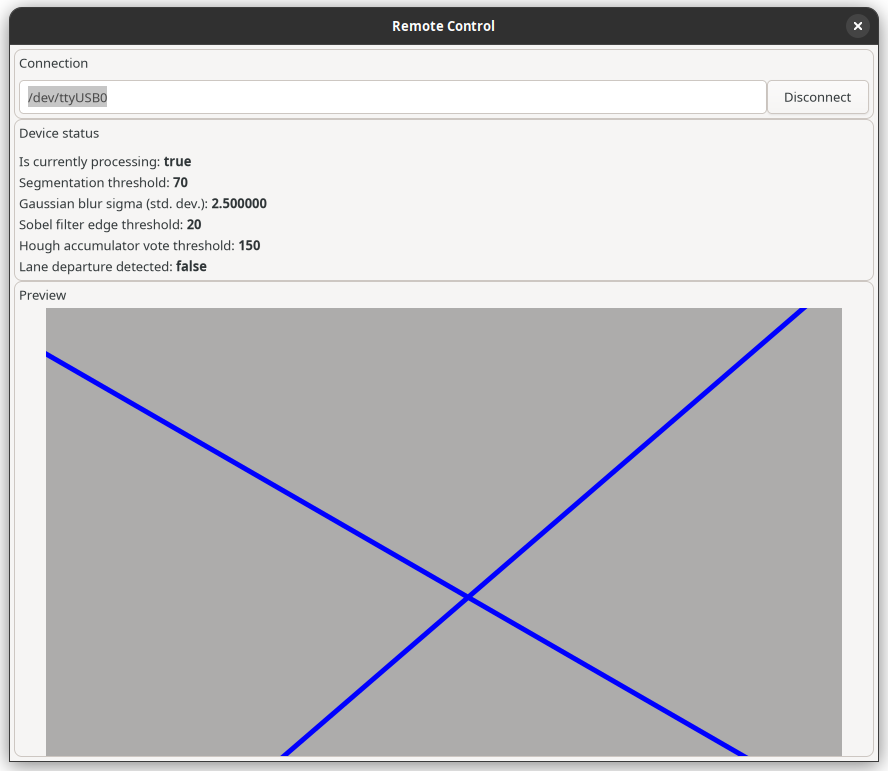
\includegraphics[width=0.845\textwidth]{product-gui.png};
			\end{figuur}
			\vspace{-1ex}

		\end{paragraaf}

		\begin{paragraaf}{Algorithm Toolsuite}

			I developed this application during the research phase of the project.
			It was my goal to get hands-on experience with the algorithms that I researched by implementing them in a computer program.
			The program is able to read/save images to disk in PPM format.
			Users can run the application from a shell, providing the path to the input image and the desired image operations by specifying the relevant command line arguments.
			I implemented the following noteworthy computer vision algorithms that I would later go on to use in the hardware lane detector:

			\vspace{-0.75ex}
			\begin{itemize}
				\item Preprocessing operations
					\vspace{-0.75ex}
					\begin{itemize}
						\item Grayscale Filter
						\item Single-channel Thresholding
						\item K-means Segmentation
						\item Gaussian Blur
					\end{itemize}
					\vspace{-0.85ex}
				\item Edge Detection operations
					\vspace{-0.75ex}
					\begin{itemize}
						\item Sobel Filter
						\item Laplacian Filter
					\end{itemize}
					\vspace{-0.85ex}
				\item Line Classification operations
					\vspace{-0.75ex}
					\begin{itemize}
						\item Hough Transform
						\item K-means Line Clustering
					\end{itemize}
					\vspace{-0.85ex}
			\end{itemize}
			\vspace{-0.25ex}

			\vspace{1.25ex}
			\begin{figuur}{Image processed using the Algorithm Toolsuite}
				\centerline{
				\begin{tabular}{ccc}
					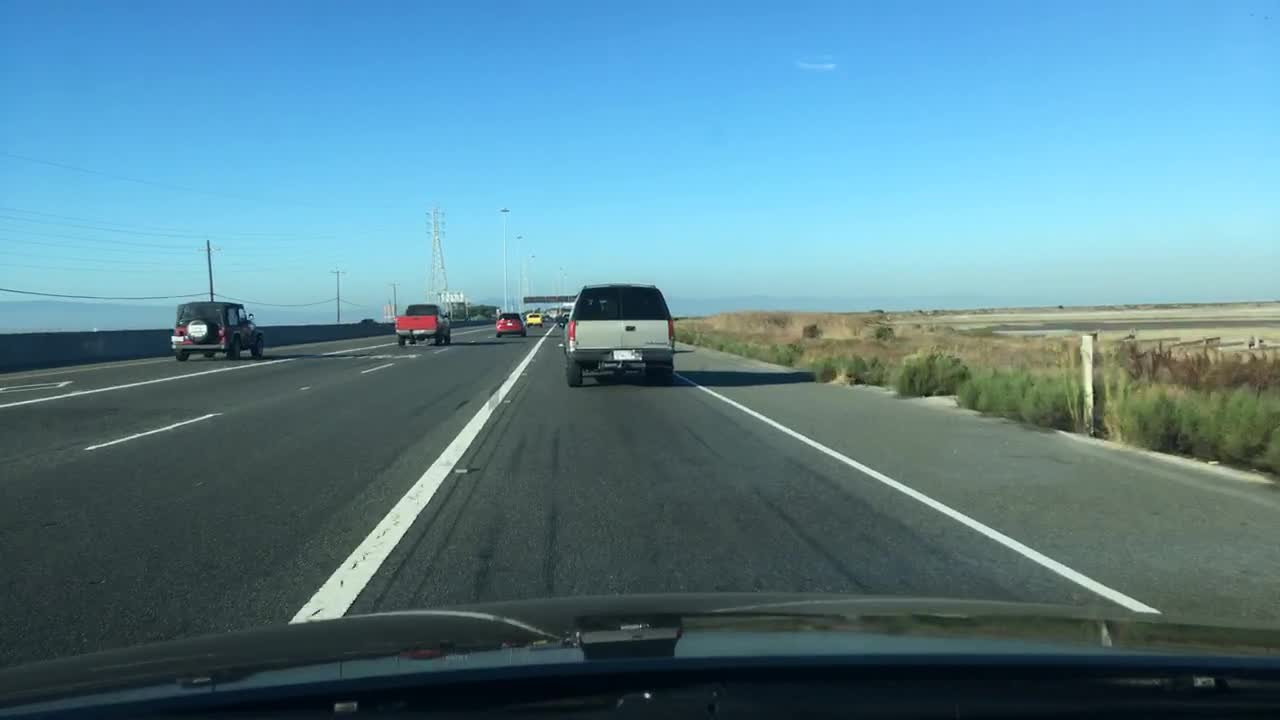
\includegraphics[width=0.475\textwidth]{0a0a0b1a-7c39d841.png} &

					\begin{tikzpicture}
						\draw[-to, white] (0, 0) -- (1, 0);
						\draw[-to, black, thick] (0, 1.65) -- (1, 1.65);
					\end{tikzpicture} &

					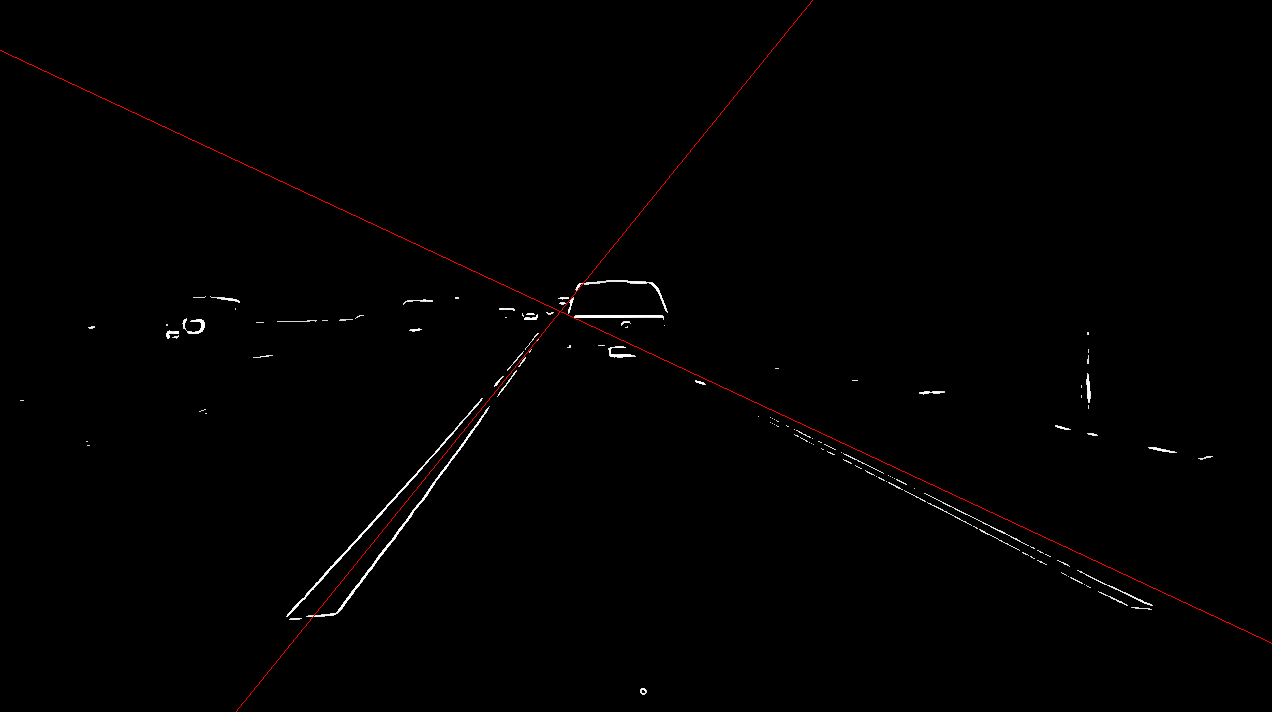
\includegraphics[width=0.475\textwidth]{0a0a0b1a-7c39d841.kmeans.out.png} \\
				\end{tabular}
				}
			\end{figuur}
			\vspace{0.5ex}
			
			\noindent An example of an image being processed with the toolsuite is given in \verwijzingb{figuur}{Image processed using the Algorithm Toolsuite}.
			The image was taken from the Berkeley DeepDrive dataset and shows an ideal scenario for detecting lane lines; the weather is clear, there is enough contrast between the paint and the road, and no major roadside artifacts are present.
			The operations performed on this image were as described in the final chapter of the research paper: first, the image is converted to grayscale and segmented into two buckets with k-means clustering.
			Then, Canny edge detection is applied to find the edge pixels in the image.
			Next, the Hough transform is applied on the edge pixels to find all the lines in the image.
			Finally, the lines are classified into lane/non-lane by using angle detection and k-means clustering.

			In the future, this program can be used to test new algorithms.
			The program can feed the entire DeepDrive database into the detection pipeline to predict its reliability.

		\end{paragraaf}

		\begin{paragraaf}{Documentation}

			Alongside the system that I built, I also wrote a lot of documentation that is valuable for the company.
			Specifically, the company is interested in how I managed to implement the detection algorithm on the FPGA.
			To document my process from design to realization, I wrote several documents that explain what steps I took, why I took them, and what decisions I made along the way.

			\begin{itemize}
				\item Advisory Report --
					In this document I reflected upon the effectiveness of the choices I made during the project, and the final benchmark results of the system. 
					I also give suggestions to the company on which steps can be taken to further improve the system and considerations that should be taken into account for potential future projects.

				\item Functional Design --
					I describe the requirements and expectations of the system.
					It is a baseline to check whether the product meets the demands that it was given.

				\item Plan of Action --
					This document described the process and planning of the project.
					It was created at the very start of the project as a guideline for working on it.
					I set out several goals for the assignment and described how I was planning to reach them.

				\item Research Paper --
					To familiarize myself with image processing and computer vision, I set out to explore different methods of lane marking detection and to compare them.
					The literature review makes up the biggest part of this paper, and looks at the different image operations in great detail.
					Mathematical constructs behind the image operations are also researched to give myself a mental picture of how the operations work.
					The practical part of the research consisted of implementing the operations myself.
					I wrote about the methods I used and the results I got, which finally led me to put together a lane marking detection pipeline.
					I used this pipeline when creating the lane detector.

				\item Technical Design --
					The goal of this document is to describe how I implemented the total system.
					I wrote about the working of each component in detail, and about how the components communicate together to form one orchestrated system.

			\end{itemize}

		\end{paragraaf}

	\end{hoofdstuk}
	
	\begin{hoofdstuk}{Management and Control}

		\setlength\parindent{1.5em}
		\setlength{\parskip}{0.5em plus 0.2em minus 0.1em}
		\linespread{1.2}
		\vspace{-2.5ex}
		
		\begin{paragraaf}{Project Management}
	
			At the start of the project, I made a Plan of Action in which I explained how I was going to manage the project and turn it into a success.
			In this document I described how I planned to approach the project, which factors would have significant impact on the process, and which obstacles I envisioned there to be.
			The plan held true for most of the project; the only major change we had to make was to switch to a different FPGA development board halfway during the project, because the original one did not have enough resources.

			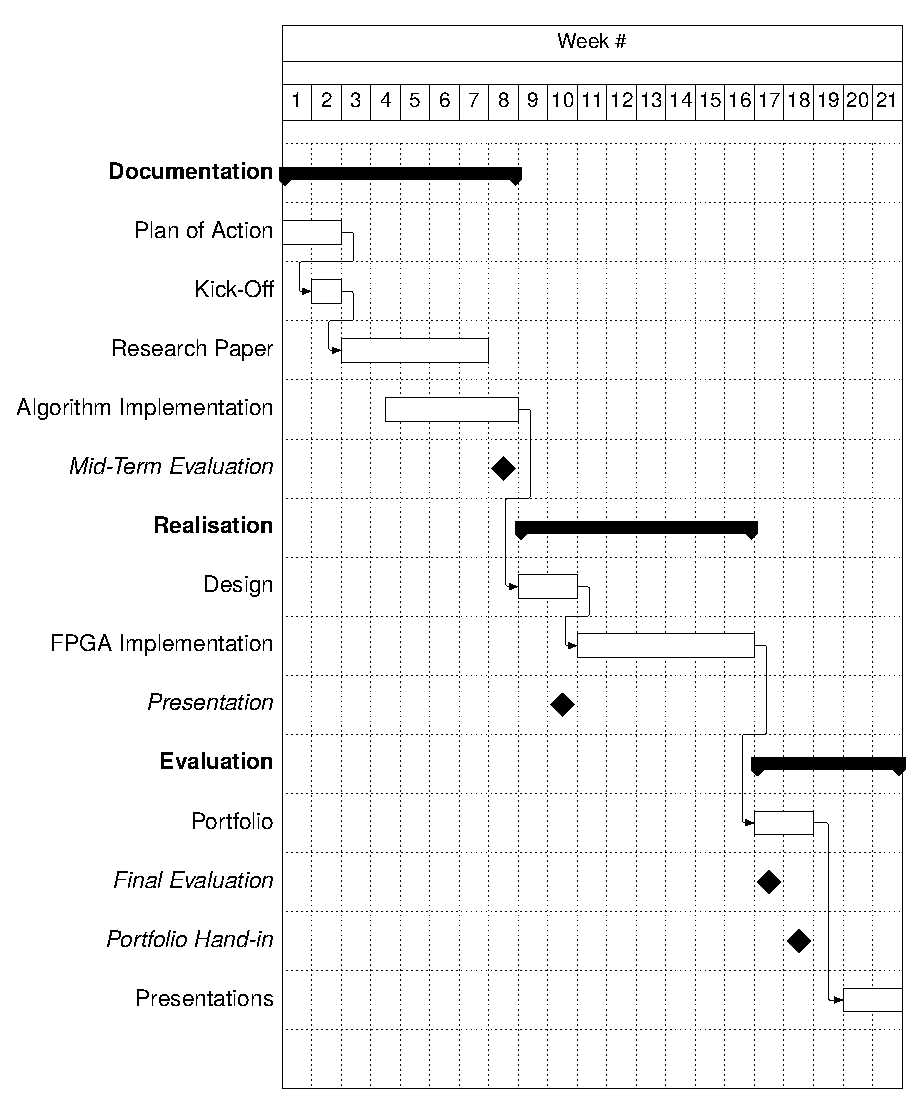
\includegraphics[width=0.8\textwidth, clip, trim=0cm 10.1cm 0cm 0cm]{planning.pdf}
			\vspace{0.25ex}

			\noindent The planning was divided into three phases: documentation, realization and evaluation.
			I started off with the documentation phase which consisted of writing the research paper and creating the test implementation.
			This phase was very important to me, because I had no prior experience with computer vision.
			By researching and implementing the relevant computer vision techniques, I taught myself the skills needed for the realization phase.
			Initially, I planned 4 weeks for the research paper and 2 weeks for the implementation, but upon recommendation from my company mentor I reallocated the time to give myself 1.5 weeks more for the implementation.
			Looking back at this decision, it was not needed because I finished the research paper earlier than expected.

			\vspace{0.65ex}
			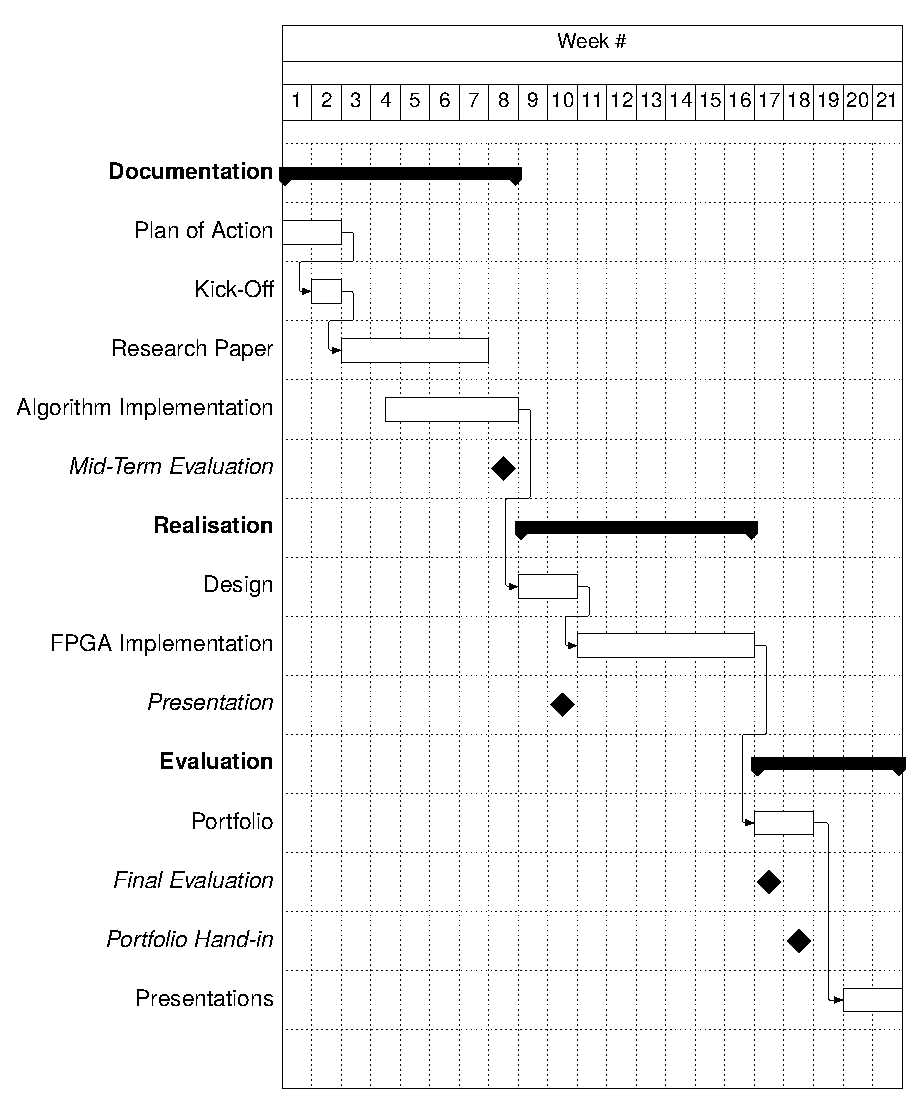
\includegraphics[width=0.8\textwidth, clip, trim=0cm 6.5cm 0cm 8.5cm]{planning.pdf}
			\vspace{0.4ex}

			\noindent I started the realization phase two weeks early due to having finished the research earlire than expected.
			I designed the system from the functional and technical perspectives, and then programmed it based on these designs.
			At the end of week 16, just as planned, I had a fully functional system and we were happy with the result.

			\noindent I wrote the advisory report and the internship report during the last phase of the project; the evaluation phase.
			Two weeks were dedicated to these activities, which were more than enough.
			Overall, I was happy with how the planning of the project turned out.
			At no point did I experience time pressure or did I feel like the project was getting out of my control.
			
			\begin{figuur}{Gantt Chart of the Planning}
				\justifying
				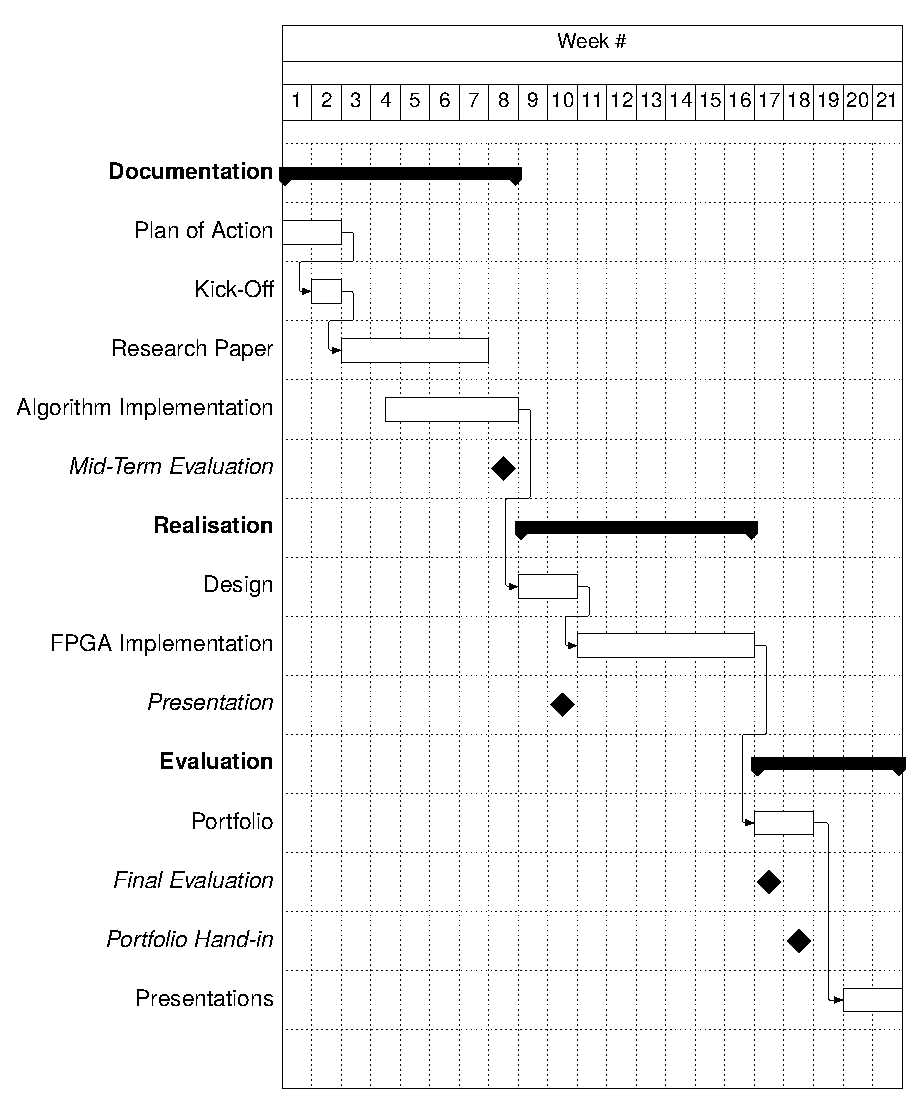
\includegraphics[width=0.8\textwidth, clip, trim=0cm 0.25cm 0cm 12.5cm]{planning.pdf}
			\end{figuur}
			
			\noindent The Plan of Action was really useful for me during the project because I used it as a guideline for what the project entailed as a whole, and what the product needed to conform to.
			During the development phase, I referred back to the Quality Management part to make sure that the code I wrote adhered to the standards I set out to follow.
			By viewing the system as a whole, I tested that the component I worked on integrated well with the others and that my changes did not break the working with other components.

			\vspace{1ex}
			\begin{figuur}{Progress Report}
				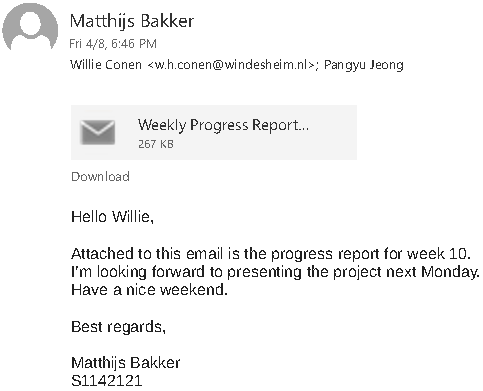
\includegraphics[width=0.6\textwidth]{progress-crop.pdf}
				\vspace{0.5ex}
			\end{figuur}

			\noindent At the end of every week, I updated the stakeholders by sending them a progress report.
			This progress report was based on the extended report template that Windesheim provided and contained all the important information, such as the hours that I worked, the activities that I worked on, and the major accomplishments I made.

		\end{paragraaf}

		\begin{paragraaf}{Agile Techniques}
			
			During previous projects at Windesheim I frequently made use of Scrum project management technique.
			I liked this technique because of how a complete and working product was created at the end of each sprint.
			The next sprint would build upon this working product to add more features, but Scrum always encouraged the developers to create a product that functioned rather than expand it into oblivion.
			I felt that a similar approach was needed for this project, because it would become complicated very quickly.
			If I didn’t focus on getting a basic functioning product, it would get complex and disjointed; I could have finished the project with nothing but individual components that could not work together.
			
			The use of these required multiple people to take accountability for different stakeholders (the product owner, the Scrum master, etc. \cite{gant2019scrum})
			Because I worked on this project alone, I wanted to try a different project management technique.
			I chose to use the Solo Iterative Process technique \cite{dorman2012sip}.
			It encourages the developer to work in iterations that are similar to Scrum sprints; the goal of an iteration is to add functionality to the product and have it functioning together at the end of this timeframe.
			Using this methodology, I set up the realization phase of the project into six incremental goals.
			Each of these goals resulted in a partial, but fully functional product which could be tested and which I could present to my company mentor:
		
			\begin{enumerate}

				\item Set up the development environment using a Makefile to automate the process and guarantee consistent results
				\item Set up communication between the board and my laptop; debugging and sending/receiving image data
				\item Create a simple grayscale filter in digital logic and process an image with it to verify that PS/PL communication works
				\item Implement the rest of the image preprocessing steps. Verify the results with the host's OpenCV program in co-simulation
				\item Implement the edge detection and Hough transform. Verify the results in co-simulation
				\item Implement smoothing and classification of the line detection results in the software driver

			\end{enumerate}

			\noindent I did not set a specific timeframe for each goal because I had no insight into how long each one would take.
			Instead, I gradually implemented each goal until I was finished. Looking back at it, I could have made a more specific planning and divided the goals into smaller tasks.
			A positive thing that I really enjoyed about this approach was that I always kept the documentation up-to-date.
			At the start of every iteration, I updated the technical documentation to reflect the current state of the product, leaving me with little to no work left after completion.

		\end{paragraaf}

		\begin{paragraaf}{Version Control}

			I used the \textit{git} version control software to keep a journal of my work.
			I kept track of all code and documentation inside a git repository (monorepo.)
			The main motivation to use git was to allow me to easily revert back to previous versions of my work and keep track of changes that I made.
			Another great feature of git (specifically GitHub, the online service I used to host my git repository) was the usage of workflows.
			They are automated testing scripts that are run on every commit to test the integrity of the code.

			The first workflow I created was one that spell-checked the documentation and compiled the LaTeX text into PDF files.
			If the documentation contained errors, like unresolved bibliography references, unresolved images, or major grammatical errors, the workflow would fail and send me an error message.
			For example, the document compilation failed on the 29th of March because I forgot to add an image asset to the git repository. I received an error, as seen in \verwijzingb{figuur}{Git Workflow Failure} and I rectified the error with another commit later that day.
			At the end of the project, I had the sources and PDFs of all documents throughout all revisions, which I used to look back upon the process.

			\begin{figuur}{Git Workflow Failure}
				\centerline{
					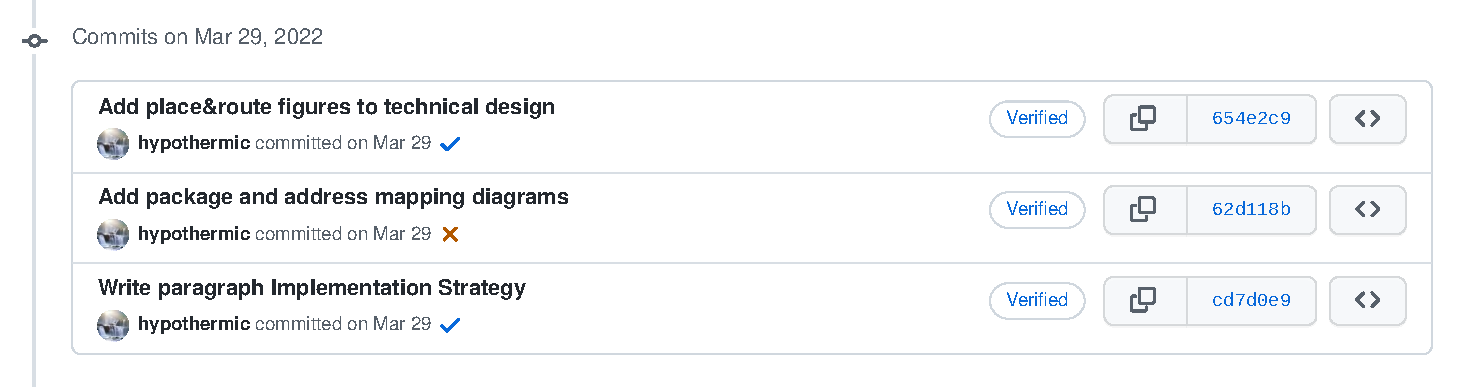
\includegraphics[width=0.55\textwidth, clip, trim=0cm 0cm 15cm 0cm]{git-commits-crop2.pdf}
					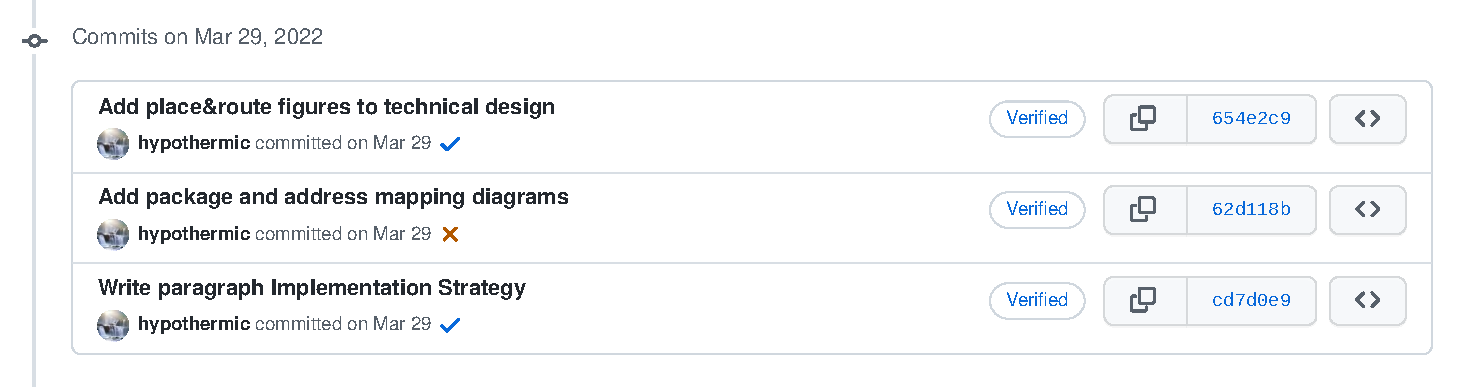
\includegraphics[width=0.55\textwidth, clip, trim=15cm 0cm 0cm 0cm]{git-commits-crop2.pdf}
					\hspace{2ex}
				}
				\vspace{-2ex}
				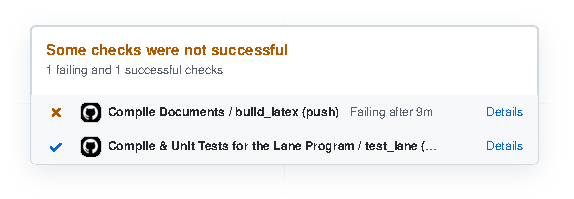
\includegraphics[width=0.9\textwidth]{git-commits-fail-crop.pdf}
				\vspace{-2.5ex}
			\end{figuur}

			\noindent I also set up a workflow for the code, which would make sure that there were no compilation warnings and that the unit tests would succeed.
			If the unit tests errored or the output was unexpected, this workflow would fail and I would receive an error report.
			The workflow automatically generated the code documentation using \textit{doxygen} and published it to a GitHub Pages website, allowing me to view it at any time.

		\end{paragraaf}

	\end{hoofdstuk}
	
	\begin{hoofdstuk}{Analysis}

		\setlength\parindent{1.5em}
		\setlength{\parskip}{0.5em plus 0.2em minus 0.1em}
		\linespread{1.2}
		\vspace{-1ex}
		
		At the start of the project, I had no experience with image processing and computer vision.
		To gain knowledge of these topics and to educate myself on what was needed to implement a lane detection pipeline, I set out to learn about relevant computer vision algorithms during the research phase of the project.
		The main question of this research paper was: \textit{"What is the best suited combination of computer vision algorithms for detecting road lane markings from a video feed?"}

		\begin{paragraaf}{Methods}

			It was vital to select an algorithm that would work well, because it would be difficult to change the algorithm after implementing it in hardware.
			Any changes that would have needed to be made would have set back the project and undone a lot of work.
			I did not want to take any chances, so I decided to thoroughly compare which detection techniques are used in the wild, and implement them in a computer program so that I could test their effectiveness.

			\begin{subparagraaf}{Literature Study}
		
				I held a literature study in which I compared the algorithms that were frequently used in other lane detection research papers, as can be seen in \verwijzingb{figuur}{Comparison of Frequently Used Algorithms among Other Researches}.
				I gathered my own knowledge on these algorithms and explained their working using my own words.
				Furthermore, I researched the mathematics behind them to help me implement all of them in a small computer program: the algorithm toolsuite.
				I used this program to evaluate the effectiveness of every algorithm and to help me string them together to compose the most effective pipeline as possible.
				
				\begin{figuur}{Comparison of Frequently Used Algorithms among Other Researches}
					\centerline{\scalebox{0.8325}{
						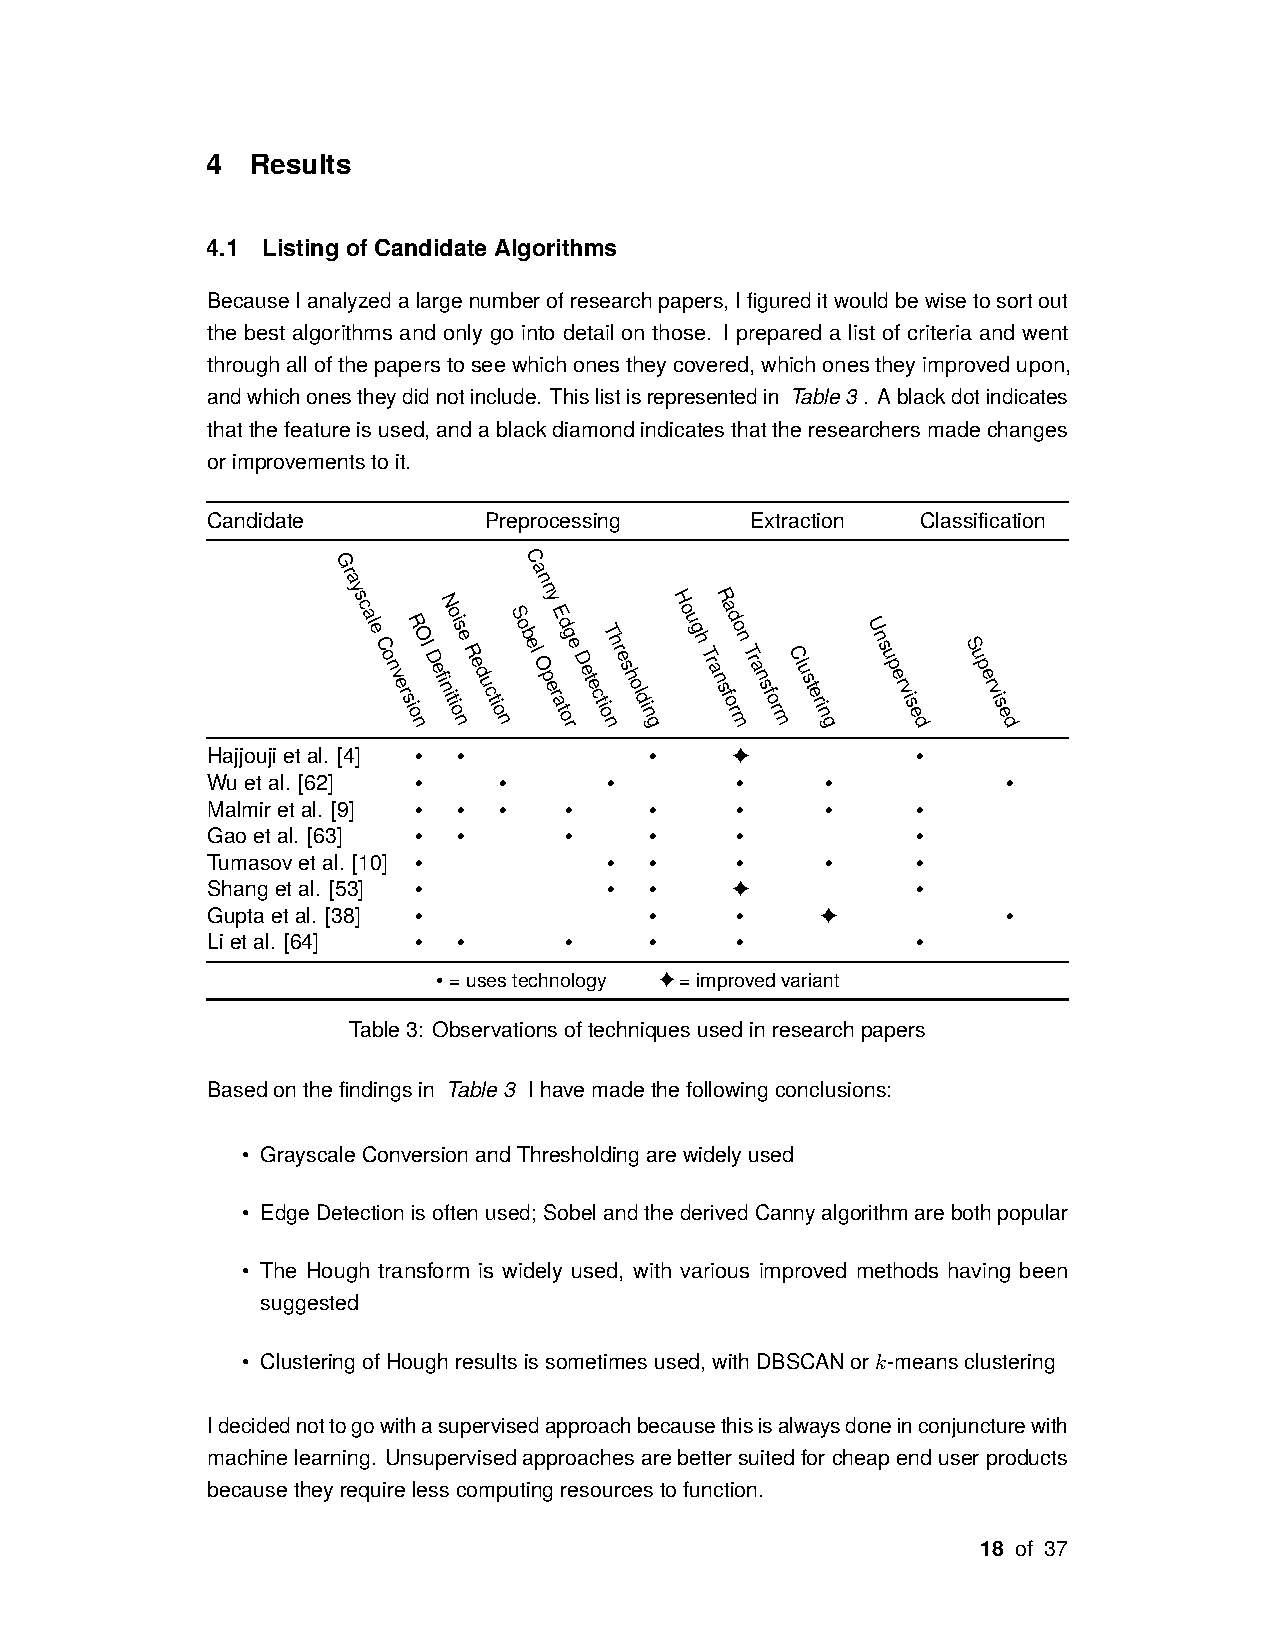
\includegraphics[clip, trim=2.75cm 10.25cm 2.75cm 8.25cm]{research-paper-conclusion.pdf}
					}}
				\end{figuur}
			
			\end{subparagraaf}

			\begin{subparagraaf}{Test Implementation}

				In order to gain familiarity with the computer vision algorithms, I implemented them in the ``algorithm toolsuite'' computer program.
				This program can load images from disk in PPM format and apply the algorithms to them, in order to test their effectiveness.
				I tested the effectiveness of the processing pipeline using the Berkeley DeepDrive dataset, which is a library of 100,000 sample images taken from dashboard cameras.
				For this, I set up a script that automatically fetched images from the dataset and fed them through the computer program.
				This testing emulated real-world scenario's to gauge the total reliability of the pipeline.
				I set up a list of criteria to judge this reliability and effectiveness.
				These criteria included the accuracy of detection in different environments, the feasibility of implementing it in digital logic, and the resources required to implement the pipeline in real-time.
				After all, it had to be possible to implement within the timeframe of the project and had to be small enough to fit on the FPGA fabric.

				\begin{figuur}{Practical Workflow of the Research Implementation}
					\centerline{\scalebox{0.8325}{
						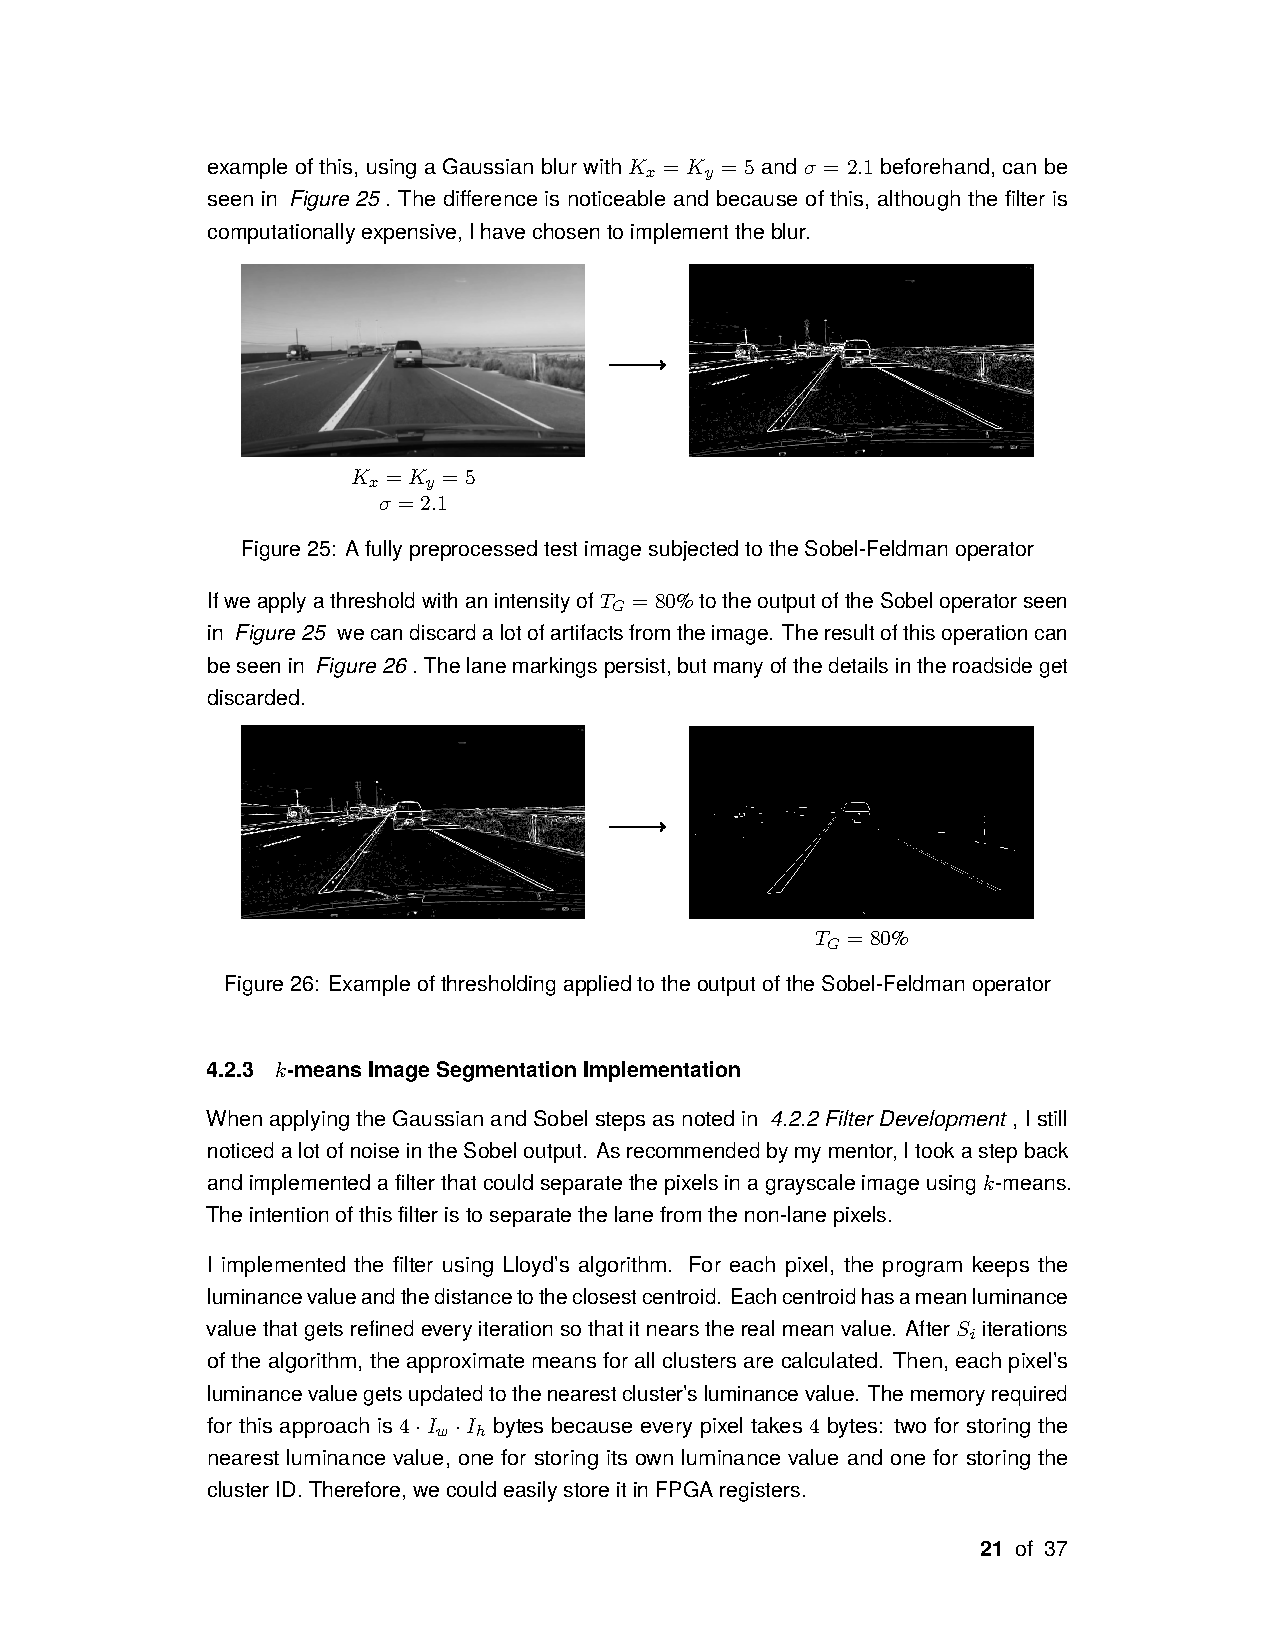
\includegraphics[clip, trim=2.75cm 11cm 2.75cm 4.1cm]{research-paper-results.pdf}
					}}
				\end{figuur}

				\noindent In the research paper I explained all the steps I took in a chronological order.
				I did this to easily express the roadblocks I hit with certain algorithms and to explain how I solved these.
				Looking back at it, this chapter of the research paper almost reads like a story, and that perfectly illustrates the learning journey I took.

			\end{subparagraaf}

		\end{paragraaf}

		\begin{paragraaf}{Results}
			
			Using the sample tests, I decided on a detection pipeline consisting of Canny edge detection and the Hough transform, along with other minor operations.
			I came to the conclusion that this pipeline was good enough for most scenarios, but my testing did indicate that it would not be effective under certain environmental conditions like sun glare, wet road surfaces, and other hazards.
			Especially when roadside objects with straight lines, like guardrails, light poles or trees were present, the results would be inaccurate because the Hough transform would pick up the lines of these arbitrary objects.
			I discussed this with my mentor and we decided that the pipeline was good enough for the project because this would only be a prototype.
			I also argumented that the pipeline would get much more complicated if we were to account for all environments, and that it would not be certain if we had enough time or resources to implement more advanced detection methods.
			We agreed to stick with the basic pipeline for this prototype.
			Reflecting back on this, I should have pursued another detection pipeline because I had many issues later in the project where it gave inaccurate results.
			I would have chosen something that involved machine learning or AI, because these algorithms can be trained to adapt better to different environments.
			FPGAs are also very well suited for neural networks, and I can't believe that I didn't think of this possibility when creating the research paper.

		\end{paragraaf}
	\end{hoofdstuk}
	
	\begin{hoofdstuk}{Advise}

		\setlength\parindent{1.5em}
		\setlength{\parskip}{0.5em plus 0.2em minus 0.1em}
		\linespread{1.2}
		\vspace{-1ex}
		
		I wrote an advisory report for AROBS to give my thoughts on the results of the current lane detection system, and to express my views on the future of using FPGA technology for this purpose.
		This advice is valuable to the company because they are looking to apply FPGA vision in more fields, so I made sure to consider the technology from different aspects.

		\begin{paragraaf}{FPGA vs GPU Accelerated Processing}

			To compare both technologies in a practical and fair way, I compared the lane detector system to an equivalent one that could be implemented on an Nvidia Jetson Nano.
			The main question for AROBS was whether it was worth investing in FPGA technology or not.
			This meant that I not only had to consider the performance and power efficiency aspects, which were obviously in favor of FPGA technology, but also the unit costs and development costs associated with the process.

			\noindent I chose the Jetson as a reference device because it is widely used in edge devices.
			I had used the device before in a KBS project at Windesheim and was familiar with how well it is able to perform.

			\begin{subparagraaf}{Processing Latency}

				Because FPGA logic is fixed, operations are run on clock pulses.
				By looking at the amount of clock cycles required to run the video processing pipeline and dividing this number by the system clock speed of 125 MHz, I was able to determine that a video frame could be processed within a total of 11.2 milliseconds.
				However, the prototyping framework that I used to test the FPGA logic added 15 milliseconds of latency on top of this.
				If AROBS wishes to develop this system further and use lower level code for the processor system, thus eliminating the need for the prototyping framework, this latency can be discarded.

				\vspace{1.5ex}
				\begin{tabel}{Performance Benchmark Results}{l @{\extracolsep{\fill}} S[table-format=3.1]S[table-format=3.1]}
					Device & {Average (ms)} & {Standard Deviation (ms)} \tabularnewline
					\midrule

					FPGA (raw)		& 11.2		& {-} 		\tabularnewline
					FPGA (co-processing)	& 26.6		& 0.443		\tabularnewline
					Reference OpenCV (CPU)	& 72.2		& 1.801		\tabularnewline
					Reference OpenCV (GPU)	& 14.2		& 0.794		\tabularnewline
					Reference Lane Program	& 382.7		& 13.81		\tabularnewline

				\end{tabel}
				
				\noindent To compare the performance with existing technology, I also estimated the time that the Nvidia Jetson would need for processing a video frame.
				I did this by running the same OpenCV code that I used in the digital logic co-simulation tests.
				This reference code ran on my laptop's iGPU, which has roughly the same specifications as the Jetson's GPU.
				The average run time per video frame for the reference code was 14.2 milliseconds.
				This is roughly 25 percent slower than the FPGA implementation.
				Another interesting test was to compare the speed against the test program I made during the research phase.
				This program ran on a single CPU core without using hardware acceleration, meaning that it was easily outclassed.

				I came to the conclusion that the FPGA implementation performed faster than a Jetson if the prototyping framework latency is not taken into account.
				But even with taking into account this latency, the FPGA implementation was still able to process the video at a speed higher than 30 frames per second, meeting the requirements of the project.
			
				\begin{figuur}{Performance Benchmark Results in a Bar Chart}
					\centerline{
						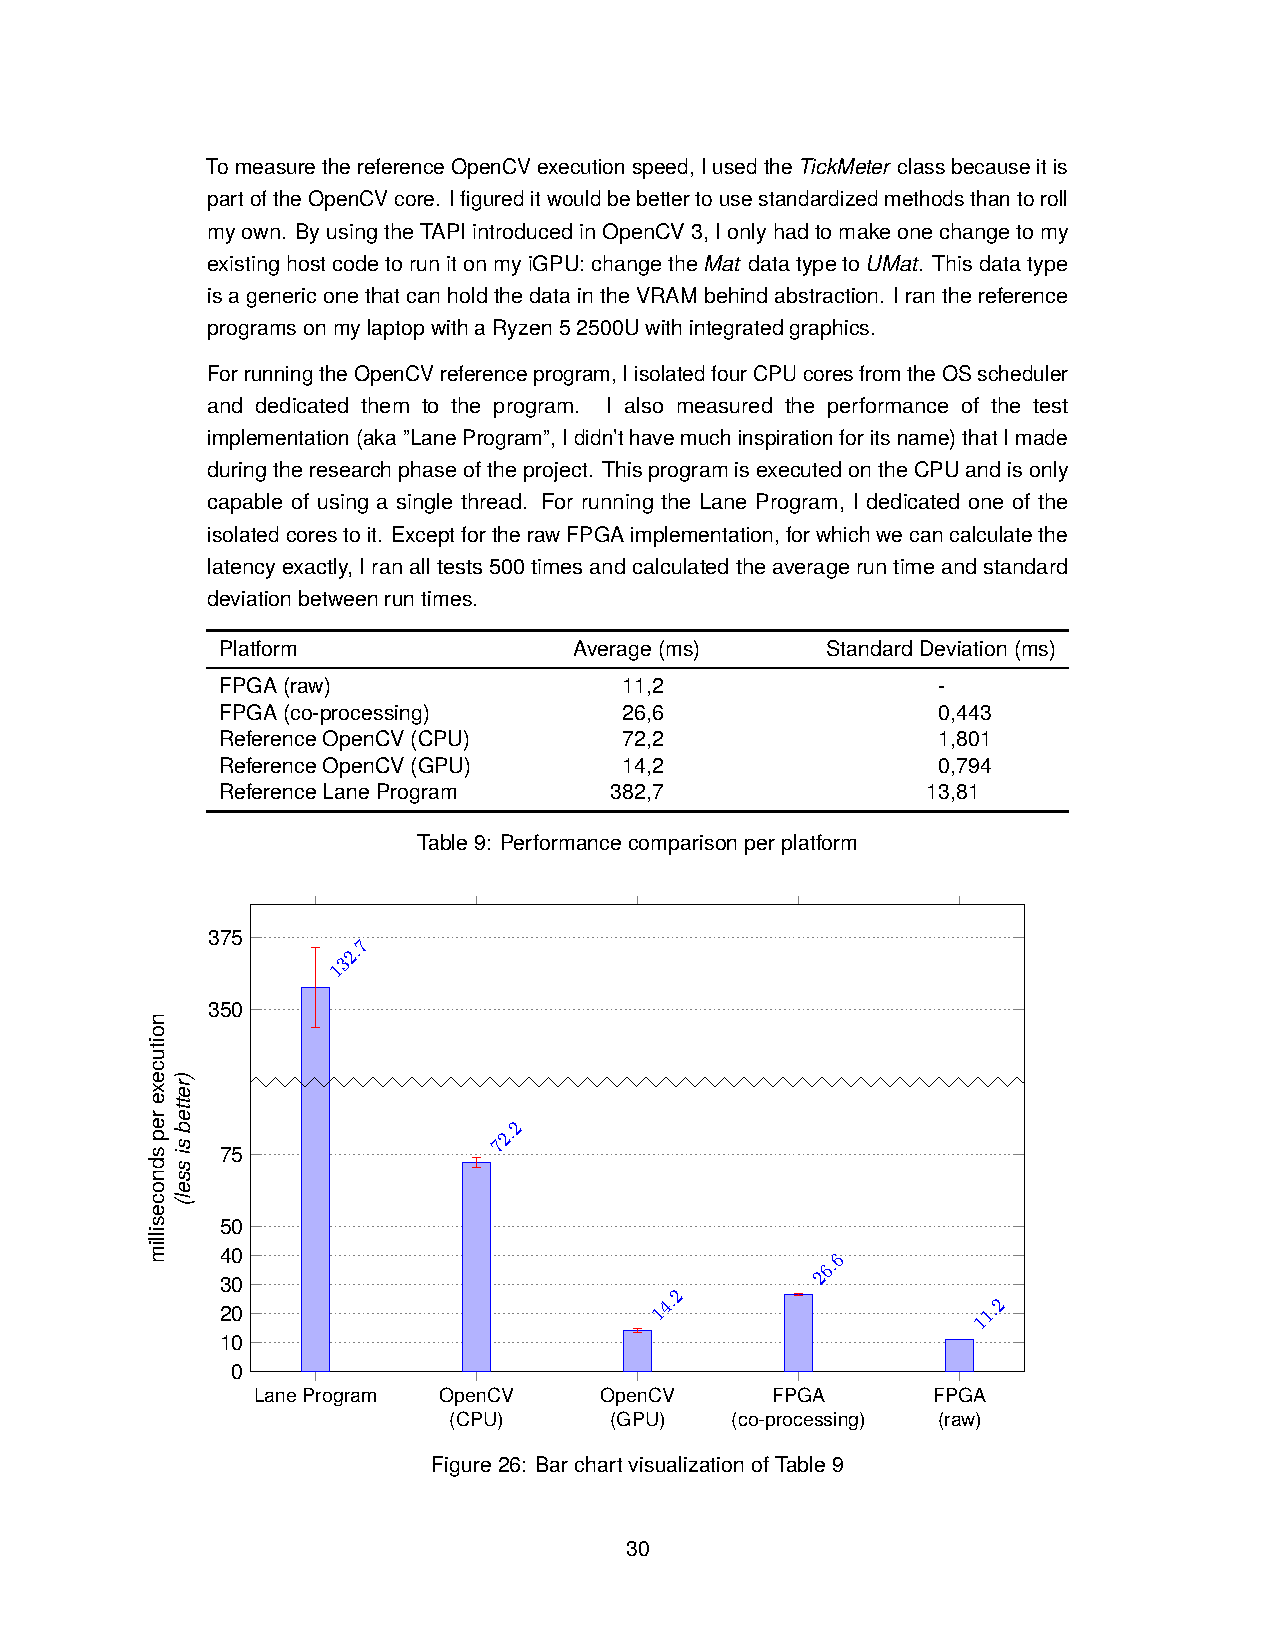
\includegraphics[clip, trim=2.5cm 3.6cm 2.5cm 15.2cm]{benchmarks.pdf}
					}
				\end{figuur}	
				\vspace{-1ex}

				\noindent I organized the results in a table, but in my opinion this did not express the difference between implementations enough.
				Therefore, I decided to plot the results next to each other in a bar chart.
				This chart shows the difference in scale of the results.

			\end{subparagraaf}

			\begin{subparagraaf}{Power Efficiency}

				One of the areas that FPGAs excel in compared to their alternatives is low power consumption.
				I measured the total chip power draw to be circa 2.25 Watt, with a fluctuation of 0.16 Watt depending on how much load was put on the CPU cores.
				The Nvidia Jetson consumes roughly 10 Watt when processing the same load.
				In the advisory report I concluded that the FPGA solution is much more suitable for being embedded in vehicles because of its low power draw.

			\end{subparagraaf}

		\end{paragraaf}

		\begin{paragraaf}{Detection Algorithm Improvement}

			Because AROBS wants to further develop this system, I gave suggestions on how the accuracy and effectiveness of the algorithm could be improved.
			The most apparent downside of the lane detector is that it does not work in some environmental conditions.
			For example, on dashcam footage where the contrast between the road and the lane markings was too low, the lane markings would simply not get detected.
			This would also happen if sun glare was captured in the lens of the camera or if the road surface was very reflective.
			Both of these defects can be solved by improving the preprocessing of the video.
			I advised AROBS to investigate more effective preprocessing methods for the video processing pipeline or to consider different approaches like the usage of a neural network.

			\vspace{1.75ex}
			\begin{figuur}{Inaccurate Detection Result due to Sun Glare}
				\centerline{
				\begin{tabular}{ccc}
					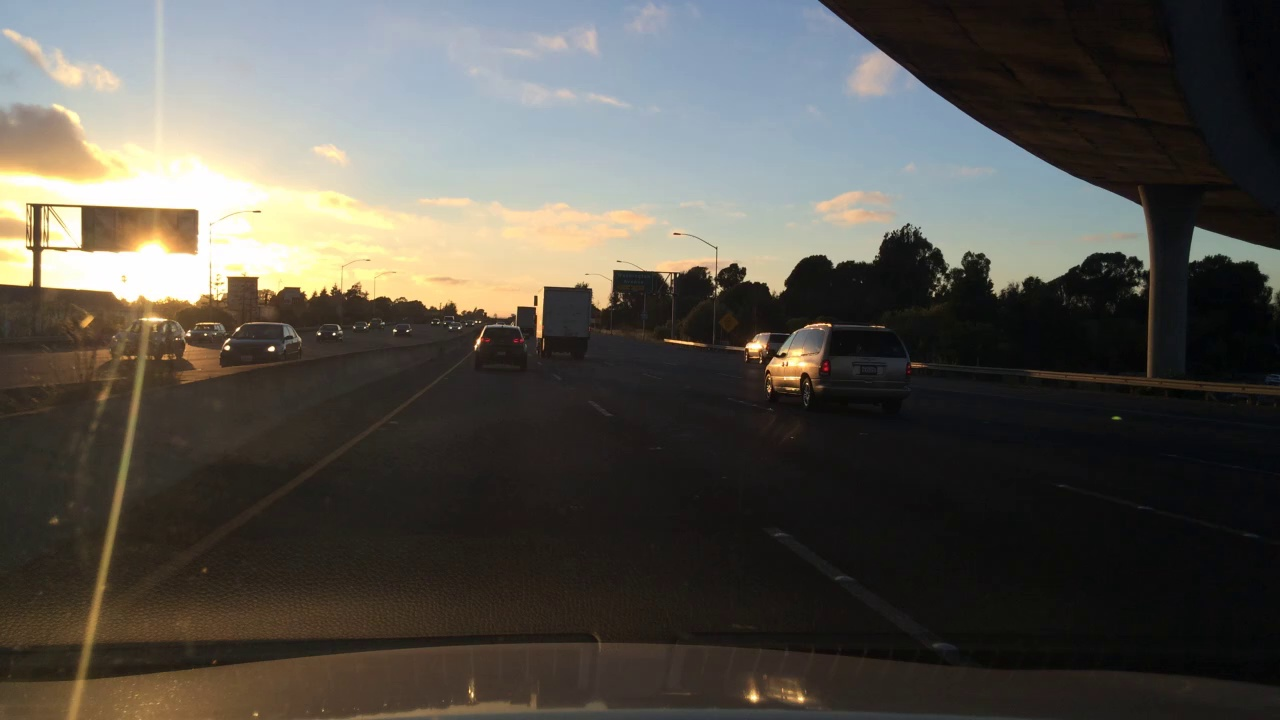
\includegraphics[width=0.475\textwidth]{0fc0b0cc-75d5e23d.jpg} &

					\begin{tikzpicture}
						\draw[-to, white] (0, 0) -- (1, 0);
						\draw[-to, black, thick] (0, 1.65) -- (1, 1.65);
					\end{tikzpicture} &

					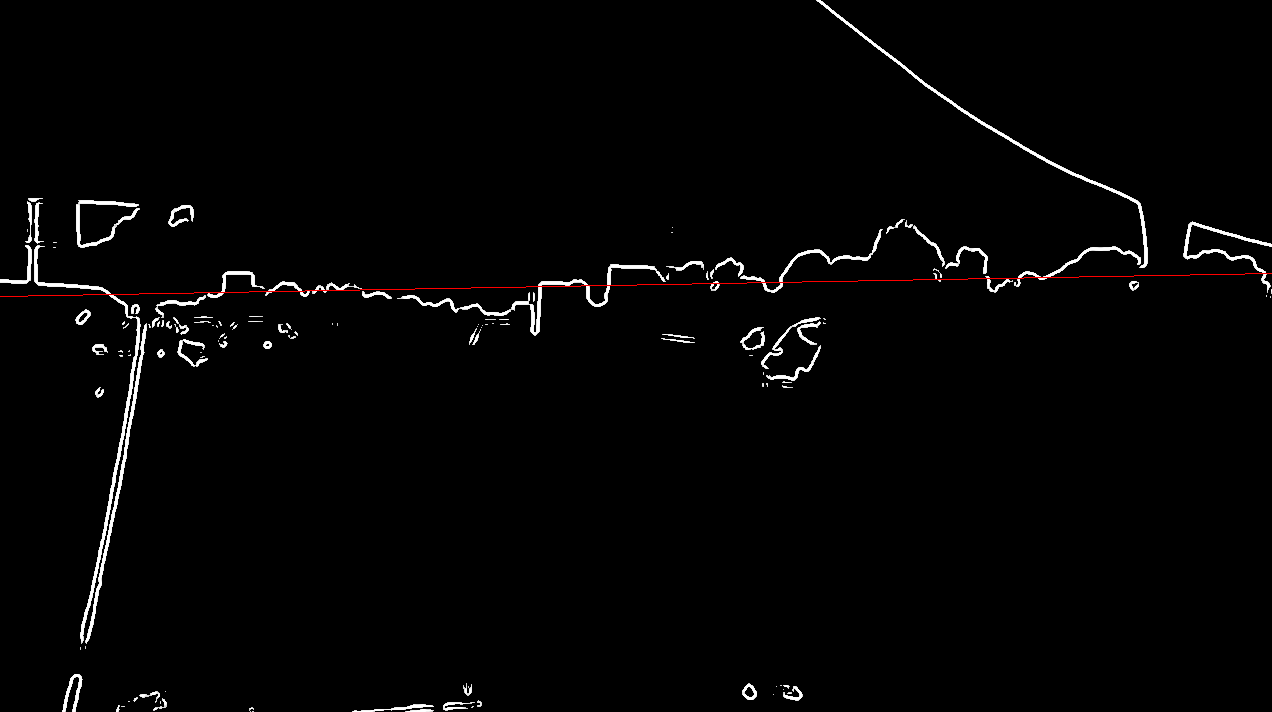
\includegraphics[width=0.475\textwidth]{0fc0b0cc-75d5e23d.grayscale.out.kmseg.out.gaussian.out.sobel.out.hough_kmeans.out.png} \\
				\end{tabular}
				}
			\end{figuur}
			\vspace{0.5ex}

			\noindent Another culprit of the lane detection algorithm is that it incorrectly classifies roadside objects with straight horizontal edges like guardrails, poles and buildings as lane lines.
			This frequently occurred in busy urban areas like in \verwijzingb{figuur}{Inaccurate Detection Result due to Roadside Artifacts}.
			I did propose several techniques to ignore these false lines in the research paper, but after discussing it with my mentor we decided not to implement them because it would hinder the flexibility of the system.
			For example, the video feed could be cropped to only include the actual road surface.
			This, however, would mean that we would need to define the crop region for each setup, and that would not make the device generic enough for any car.
			To keep the prototype system as universal as possible, we decided against these optimizations, but considering the poor accuracy of the lane detection, I advised AROBS to look into these improvements again.

			\vspace{1.75ex}
			\begin{figuur}{Inaccurate Detection Result due to Roadside Artifacts}
				\centerline{
				\begin{tabular}{ccc}
					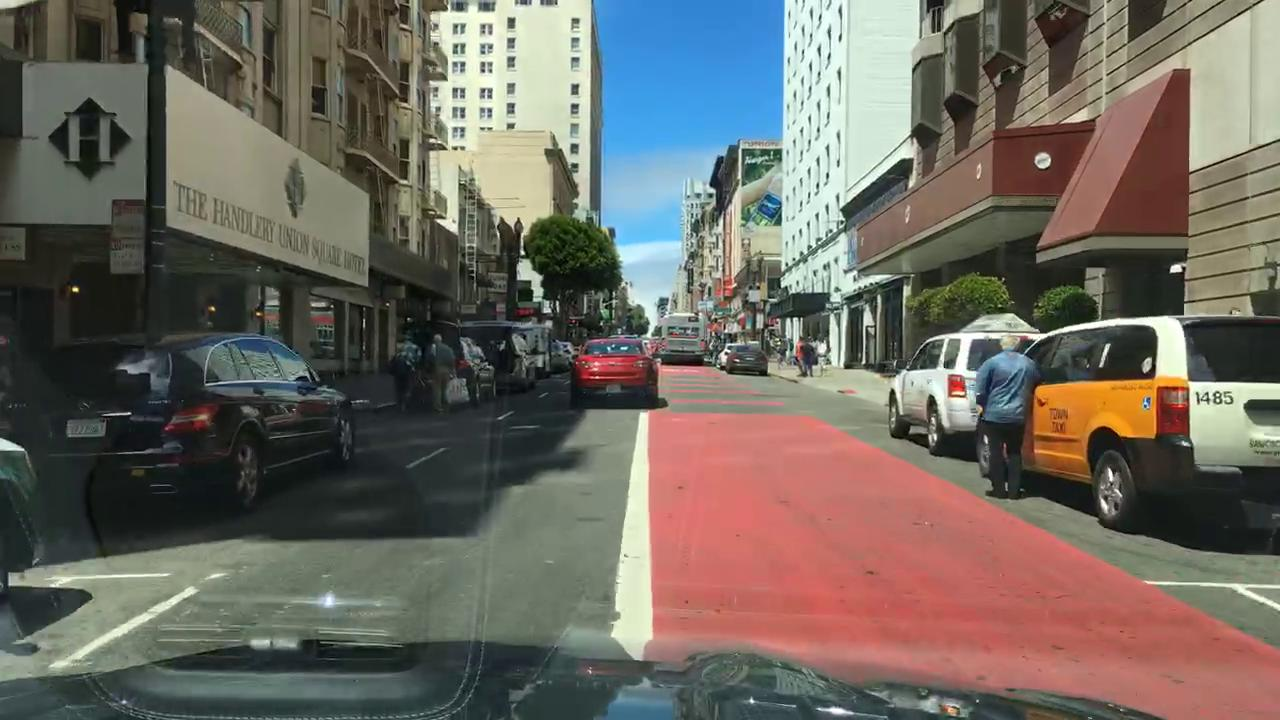
\includegraphics[width=0.475\textwidth]{0f1a2d28-bfa30000.jpg} &

					\begin{tikzpicture}
						\draw[-to, white] (0, 0) -- (1, 0);
						\draw[-to, black, thick] (0, 1.65) -- (1, 1.65);
					\end{tikzpicture} &

					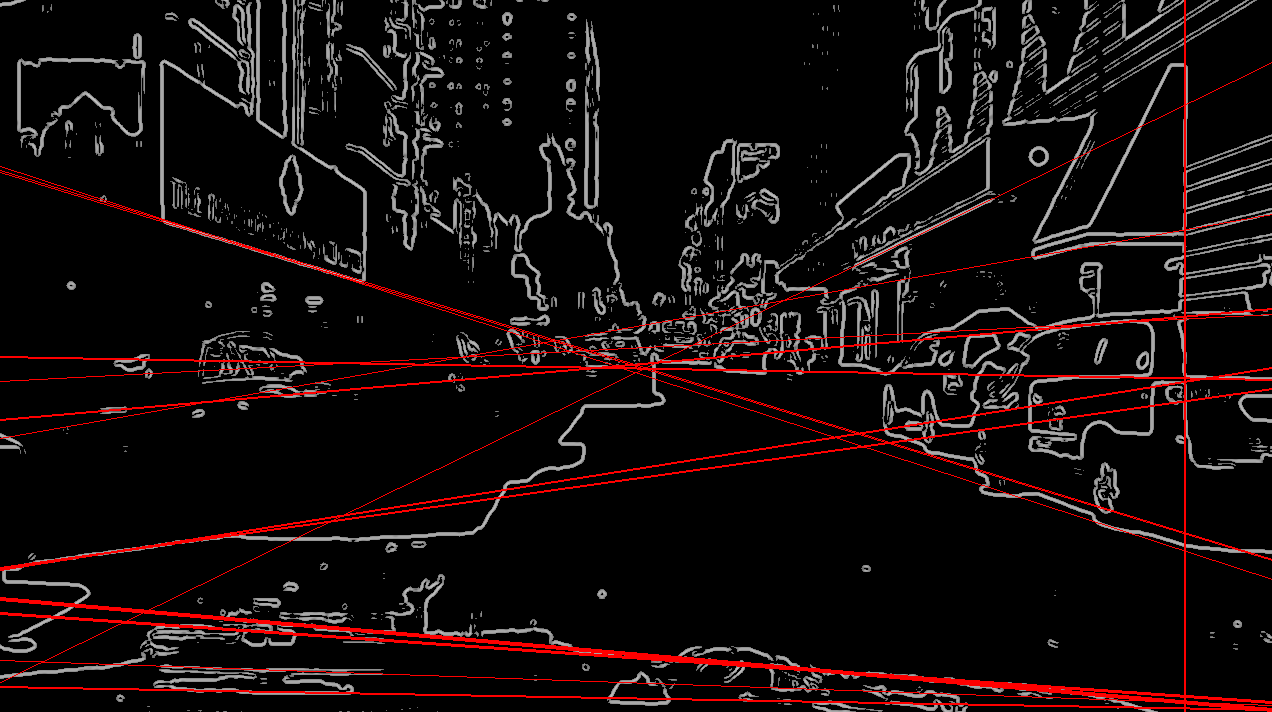
\includegraphics[width=0.475\textwidth]{0f1a2d28-bfa30000.grayscale.out.kmseg.out.gaussian.out.sobel.out.hough_overlay.out.png} \\
				\end{tabular}
				}
			\end{figuur}
			\vspace{0.5ex}
		\end{paragraaf}

	\end{hoofdstuk}
	
	\begin{hoofdstuk}{Design}

	\end{hoofdstuk}
	
	\begin{hoofdstuk}{Implementation}

	\end{hoofdstuk}
	
	\begin{hoofdstuk}{Professional Development}

	\end{hoofdstuk}

	% Bibliography page
	\begin{hoofdstuk}{References}

		\printbibliography[heading=none]

	\end{hoofdstuk}

	\makelastpage

\end{document}

